\documentclass[11pt]{article}
\usepackage[utf8]{inputenc}
\usepackage{amsmath}
\usepackage{amssymb}
\usepackage{amsthm}
\usepackage{tcolorbox}
\usepackage{tikz}
\usetikzlibrary{positioning}
\usepackage{graphicx}
\usepackage{natbib}
\usepackage{bibentry}
\usepackage[nottoc]{tocbibind}
\usepackage{mathrsfs}
\usepackage{subfigure}
\usepackage[font=small,labelfont=bf]{caption}
\usepackage{mathtools}

\usetikzlibrary{fit}
\mathtoolsset{showonlyrefs}
\bibliographystyle{plainnat}
\numberwithin{equation}{section}

\newcommand{\argmax}[1]{\underset{#1}{\operatorname{arg}\,\operatorname{max}}\;}
\newcommand{\KL}[2]{\text{KL}\left(#1 \vert\vert #2\right)}
\newcommand{\expectation}[1]{\mathbb{E}\left[#1\right]}
\newcommand{\Tr}[1]{\text{Tr}\left(#1\right)}
\newcommand{\x}{{\bf x}}
\newcommand{\X}{{\bf X}}
\newcommand{\z}{{\bf z}}
\newcommand{\Z}{{\bf Z}}
\newcommand{\N}{\mathcal{N}}
\newcommand{\R}{\mathbb{R}}

\newtheorem{definition}{Definition}[section]
\newtheorem{proposition}{Proposition}[section]
\newtheorem{theorem}{Theorem}[section]

% In this dissertation/project we formalise the derivation of the Kalman Filters' equations from the perspective of a state-space model
% We show that the Kalman Filters equations arise 
% as the E-step of the EM-algorithm applied to a Linear Dynamical System with added noise.
% Furthermore, we test the limitation of the Kalman Filter algorithm to recover 

\title{Probabilistic Linear Dynamical Systems}
\author{Gerardo Durán-Martín}
\begin{document}
\allowdisplaybreaks
% Add everything to bibliography, even if it is not cited.
\nocite{*}

\maketitle

\section{Introduction}

Dynamical systems are models that capture the time evolution of a system (\cite{strogatz}). A discrete-time linear dynamical system is a $K$-dimensional vector $\z_n$ which evolves according to a real-valued matrix ${\bf A}\in\R^{K\times K}$ in the form

\begin{equation}
	\z_{n+1} = {\bf A}\z_n.
\end{equation}

Figure \ref{fig:discrete-dynamical-system} shows an example of discrete dynamical, which starts at the state $\x_0$ and ends in the state $
\x_{18}$.

% An example of a linear dynamical system is...
\begin{figure}[h!]
	\centering
	\includegraphics[scale=0.5]{../figures/discrete-dynamical-system}
	\caption{Example of a discrete-time dynamical system.}
	\label{fig:discrete-dynamical-system}
\end{figure}



In this work, we are interested in dynamical systems that depend on unobserved values, usually called latent variables, and on a set of observed values that are directly derived from the source signal. We define the set of observed variables $\X = \{\x_n \in \mathbb{R}^M \vert n=1,\ldots, N\}$ as the observed dataset, and the set of latent variables $\Z = \{\z_n \in \mathbb{R}^K \vert n=1,\ldots, N\}$ as the latent dataset. We will use $\mathcal{D} = ({\bf X}, {\bf Z})$ to denote the complete-dataset.

A linear dynamical system with latent variables assumes the existence of an unobserved signal $\z_n \in \mathbb{R}^K$ that evolves linearly over time according to a matrix ${\bf A}\in\mathbb{R}^{K\times K}$. Once $\z_{n+1}$ is obtained, the observed value $\x_{n+1} \in \mathbb{R}^M$ is the result of a linear transformation over $\z_{n+1}$ induced by the matrix ${\bf C}\in \mathbb{R}^{M\times K}$. The equations that govern such a system can be written as follows:

\begin{align*}
	\z_{n+1} &= {\bf A} \z_{n},\\
	\x_{n+1} &= {\bf C} \z_{n+1}.
\end{align*}

An example of such a system is presented in Figure \ref{fig:hidden-dynamical-system}, in which the dynamics of the vector $\x_n$ are completely determined by the vector $\z_n$. Hence, the evolution of the system is specified by the initial condition $\z_0$. Assuming that $\z_0$ is known and we observe a fixed number $N$ of observations, the problem reduces to find matrices ${\bf A}$ and ${\bf C}$ that generate the observed values.

\begin{figure}[h!]
	\centering
	\includegraphics[scale=0.5]{../figures/hidden-dynamical-system}
	\caption{Example of a hidden dynamical system. The blue arrows represent the underlying (hidden) system, whereas the orange arrows the observed system.}
	\label{fig:hidden-dynamical-system}
\end{figure}

In some settings, however, we assume that the underlying signal $\z_n$ and the observed value $\x_n$ do not behave deterministically. Suppose, for example, that we are interested in modelling the price of a stock. We would like to determine whether the price of the stock is likely to go up or down. To determine its trajectory, we assume that the stock has an underlying price that consists of natural fluctuations. Furthermore, market forces such as speculation, false information, or irrational behaviour may move the underlying price of the stock to higher or lower levels and add additional noise to the observed price. Our goal is to recover the underlying price of the stock by \textit{filtering out} the fluctuation introduced by the market and the natural fluctuation (see Figure \ref{fig:1d-stock-system}). 

Hence, in Panel (a), we observe that the underlying price of the stock oscillates around a mean price, whereas in {Panel (b) the observed market price closely follows the underlying price with an additional noise.

\begin{figure}[h!]
	\hfill
	\subfigure[Underlying price]{\includegraphics[width=6cm]{../figures/underlying-price}}
	\hfill
	\subfigure[Observed price]{\includegraphics[width=6cm]{../figures/observed-price}}
	\hfill
	\caption{One-dimensional linear dynamical system. Panel (a) shows the underlying price of a stock. Panel (b) shows the observed market price. In both Panels, we show the mean price of the stock that we are interested in recovering (dashed line).}
	\label{fig:1d-stock-system}
\end{figure}



More generally, let $\X = \{\x_n \in \mathbb{R}^M \vert n=1,\ldots, N\}$ be an observed dataset and $\Z =  \{\z_n \in \mathbb{R}^K \vert n=1,\ldots, N\}$ a latent dataset. We assume that each value $\x_n$ is generated by applying a function $f:\R^K\to R^M$ to a latent variable $\z_n$ plus a noise term, i.e., $\x_n = f(\z_n) + \boldsymbol\varepsilon_n$. Furthermore, each latent variable $\z_n$ is generated via a function $g:\R^K\to\R^K$ of its previous value plus a noise term, i.e., $\z_n = g(\z_{n-1}) + \boldsymbol{\varphi}_n$. Our goal is twofold: obtain a procedure that describes the noiseless mean behaviour of $\z_n$, and a technique to determine $f$ and $g$.

In this work, we show that if the proposed functions $f$ and $g$ are linear, and the noise terms are zero-mean Gaussian random variables, we can make use of the so-called Expectation Maximisation (EM) algorithm to determine $f$ and $g$, and estimate the underlying latent dataset $\Z$ using a procedure known as Kalman Filtering.

Throughout this work every random variable is taken to be real-valued. To be specific, for every $n$, $\z_n \in \R^K$ and $\x_n \in \R^M$. To reduce clutter in the notation, every integral  symbol in this work assumes a definite integral over the real numbers with dimension specified by the differential term.

\section{Linear dynamical systems with added noise}
We begin this section by formalising our model of interest. For an $M$-dimensional Gaussian distribution we have $p(\z) = \mathcal{N}(\z \vert {\bf m}, {\bf S})$ with
\begin{align}
	p(\z) &= \N(\z \vert {\bf m}, {\bf S})\\
		  &= (2\pi)^{-M/2} \vert {\bf S}\vert^{-1/2}\exp\left(-\frac{1}{2}(\z - {\bf m})^T{\bf S}^{-1}(\z - {\bf m})\right).
\end{align}
Let $g(\z_{n-1}) = {\bf A} \z_{n-1}$ with ${\bf A}\in\R^{K\times K}$, and $f(\z_n) = {\bf C} \z_{n}$ with ${\bf C} \in \R^{M \times K}$. 
Assume that a latent state $\z_n$, for $n \geq 2$, and any state $\x_n$ are each corrupted by zero-mean gaussian noise with covariance matrices $\boldsymbol{\Sigma} \in \mathbb{R}^{K \times K}$, and $\boldsymbol{\Gamma} \in \mathbb{R}^{M \times M}$ respectively. We define a  probabilistic Linear Dynamical System (pLDS) as follows:
\begin{align}
	p(\z_{n+1} \vert \z_n) &= \N(\z_{n+1} \vert {\bf A}\z_n, \boldsymbol\Gamma),\\
	p(\x_{n+1} \vert \z_{n+1}) &= \N(\x_{n+1} \vert {\bf C}\x_n, \boldsymbol\Sigma).
\end{align}
In addition, we assume that the initial state of the system $\z_1$ is normally distributed with mean $\boldsymbol{\mu}_0$ and covariance matrix ${\bf V}_0$, i.e,
\begin{equation}
	p(\z_1) = \N(\z_1 \vert \boldsymbol\mu_0, {\bf V}_0).
\end{equation}
A simulation of the evolution of such a system is presented in Figure \ref{fig:hidden-noisy-dynamical-system}, where the deterministic dynamics are the same of Figure \ref{fig:hidden-dynamical-system}.

\sloppy As we can see from the model specification, the overall dynamics of the system are completely specified by the set of parameters $\boldsymbol\theta = \{{\bf A}, {\bf C}, \boldsymbol\Gamma, \boldsymbol\Sigma, \boldsymbol\mu_0, {\bf V}_0\}$. In this work, we take a frequentist approach and find the set of parameters $\boldsymbol\theta$ that best represents the complete dataset $(\X, \Z)$. This is usually done by maximising the log-likelihood of the data with respect to each of the parameters in $\boldsymbol{\theta}$. Maximising the log-likelihood of a pLDS, however, is not straightforward. The computation of a complete-data log-likelihood, $\log p(\X, \Z \vert \theta)$, requires knowing the terms $\X$ and $\Z$ in advance. Since we are only given $\X$, we require a procedure to estimate the latent dataset $\Z$. In the following two subsections, we develop a framework to work with the joint distribution of our pLDS model, and a procedure to estimate the latent dataset $\Z$ and maximise the log-likelihood over the complete-dataset.


\begin{figure}[h!]
	\centering
	\includegraphics[scale=0.5]{../figures/hidden-stochastic-dynamical-system}
	\caption{Example of a hidden dynamical system with added noise. The deterministic dynamics of the model are the same as the ones presented in Figure \ref{fig:hidden-dynamical-system}, however, each state is corrupted with multivariate-gaussian noise.}
	\label{fig:hidden-noisy-dynamical-system}
\end{figure}


\subsection{Probabilistic Graphical Models}
A useful way to analyse the structure of joint distributions over random variables is by representing the dependencies of the joint distribution as a probabilistic graphical model. In this subsection, we define and motivate the use of Bayesian networks, and the conditional independence. Moreover, we provide the rules of $d$-separation, and postulate a set of factorisation equations that helps us analyse pLDSs. For an in-depth overview of probabilistic graphical models, see \cite{koller2009}, or Chapter 8 of \cite{prml}.

% The main subject in this subsection is to motivate the use of graphs for representing the joint distribution over random variables. 
Suppose $a$, $b$, and $c$ are random variables with marginal probability density function given by $p(a)$, $p(b)$, and $p(c)$ respectively. Depending on the relationship between each pair of random variables, the joint distribution $p(a,b,c)$ could be written differently. For example, if we assume that every node is independent of each other node, $p(a,b,c) = p(a) p(b) p(c)$. A Bayesian network is a graphical representation of the joint distribution of a set of random variables that expresses conditional relationships.

\begin{definition}
	A \textbf{Bayesian network} is a directed graph $\mathcal G = \{\mathscr{N}, \mathscr{E}\}$ with nodes $\mathscr{N}$ corresponding to a set of random variables, and edges $\mathscr{E}$ of directed links (ordered tuples) between two nodes. Edges in a Bayesian network represent causal relationships between the nodes.
\end{definition}

% provide two or three examples of factorisation using bayesian networks
To understand the use of Bayesian networks, consider $\mathcal G = \{\{a, b, c\}, \{\}\}$. Then, the joint probability over the random variables $a$, $b$, and $c$ induced by $\mathcal G$ is given by $p(a,b,c) = p(a) p(b) p(c)$. The graphical representation of $\mathcal G$ is shown in Figure \ref{fig:bayes-net-1}.

\begin{figure}[h!]
	\centering
	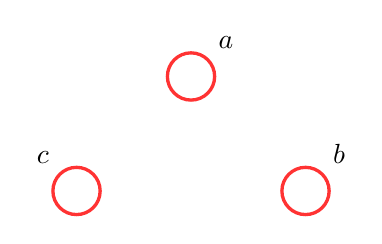
\begin{tikzpicture}[
latentnode/.style={circle, draw=red!80, minimum size=6mm, very thick},
observednode/.style={circle, draw=red!80, fill=cyan!60, minimum size=6mm, very thick},
]

% Defining the nodes
\node[latentnode, label=above right:{$a$}] (a) {};
\node[latentnode, label=above right:{$b$}] (b) [below right=of a] {};
\node[latentnode, label=above left:{$c$}] (c) [below left=of a] {};


% Relationships between latent variables

\end{tikzpicture}
	\caption{Graphical representation of the factorisation $p(a,b,c) = p(a) p(b) p(c)$.}
	\label{fig:bayes-net-1}
\end{figure}

On the contrary, if $\mathcal G = \{\{a,b,c\}, \{\{a, b\}, \{a, c\}, \{b, c\}\}\}$, the joint probability induced by $\mathcal G$ is given by  $p(a,b,c) = p(a)p(b \vert a)p(c \vert a, b)$. The graphical representation of $\mathcal G$ is shown in Figure \ref{fig:bayes-net-2}.

\begin{figure}[h!]
	\centering
	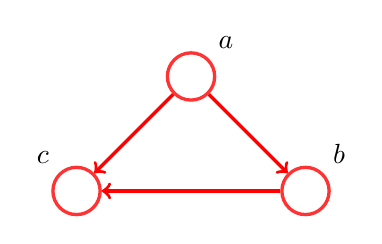
\begin{tikzpicture}[
latentnode/.style={circle, draw=red!80, minimum size=6mm, very thick},
observednode/.style={circle, draw=red!80, fill=cyan!60, minimum size=6mm, very thick},
]

% Defining the nodes
\node[latentnode, label=above right:{$a$}] (a) {};
\node[latentnode, label=above right:{$b$}] (b) [below right=of a] {};
\node[latentnode, label=above left:{$c$}] (c) [below left=of a] {};


% Relationships between latent variables
\draw[->, color=red, very thick] (a) -- (b);
\draw[->, color=red, very thick] (a) -- (c);
\draw[->, color=red, very thick] (b) -- (c);

\end{tikzpicture}
	\caption{Graphical representation of the factorisation $p(a,b,c) = p(a) p(b \vert a) p(c \vert a, b)$.}
	\label{fig:bayes-net-2}
\end{figure}


% then, define the joint distribution over graphical models
More formally, we have the following definition
\begin{definition}
	The joint distribution over a set of random variables $\x = (x_1, \ldots, x_K)$ induced by a Bayesian network is given by the product over each node in the graph conditioned on the variables corresponding to the parents of that node in the graph. It can be represented as
	\begin{equation}
		p({\bf x}) = \prod_{k=1}^K p(x_k \vert \text{Pa}_k),
	\end{equation}
	where $\text{Pa}_k$ is the set of nodes that directly influence $x_k$.
\end{definition}

It is important to remark that the Bayesian networks considered in this work cannot be strongly connected, i.e., there cannot exist a closed loop in the graph. In that sense, any Bayesian network can be represented as a Directed Acyclic Graph (DAG).

% Then, talk about the use of latent variables and the representation in a bayesian network
% * Use the pLDS as an example to write the complete-data likelihood, and
% * Write it as a probabilistic graphical model
Given any Bayesian network, it is of interest to ask how does the factorisation in a graph changes if a set of random variables are conditioned on another nonintersecting set of random variables. Conditional probabilities allow us to find simpler representations of conditional probabilities which simplifies the model and results in more efficient computations. Consider the following definition


% Then, write about conditional independence and why it is useful: to simplify the structure of a model and reduce the amount of computations required to perform learning and inference
\begin{definition}
	\textbf{Conditional independence}: Two random variables, $a$ and $b$, are said to be conditionally independent over a third random variable $c$, denoted as $a \perp b \vert c$, if the following formula holds
	\begin{equation}
		a \perp b \vert c \iff p(a, b \vert c) = p(a \vert c) p(b \vert c).
	\end{equation}
	Equivalently,
	\begin{equation}
		a \perp b \vert c \iff p(a \vert b, c) = p(a \vert c).
	\end{equation}
\end{definition}

Given a Bayesian network, in Figure \ref{fig:bayes-net-3}, we graphically denote observed random variables as nodes filled in blue. 

\begin{figure}[h!]
	\centering
	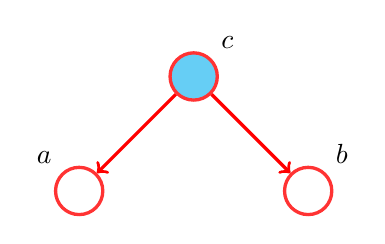
\begin{tikzpicture}[
latentnode/.style={circle, draw=red!80, minimum size=6mm, very thick},
observednode/.style={circle, draw=red!80, fill=cyan!60, minimum size=6mm, very thick},
]

% Defining the nodes
\node[observednode, label=above right:{$c$}] (a) {};
\node[latentnode, label=above right:{$b$}] (b) [below right=of a] {};
\node[latentnode, label=above left:{$a$}] (c) [below left=of a] {};


% Relationships between latent variables
\draw[->, color=red, very thick] (a) -- (b);
\draw[->, color=red, very thick] (a) -- (c);

\end{tikzpicture}
	\caption{Graphical representation of the conditional probabilty $p(a, b\vert c) = p(a \vert c) p(b \vert c)$.}
	\label{fig:bayes-net-3}
\end{figure}


% Next, write about d-separation: determine conditional independence properties directly from the bayes' net
% * Write the d-separation as a theorem (and a reference to a proof)
The distinction between observed and unobserved nodes in a network allows us to specify more complex probabilistic models that have \textit{observed} and \textit{latent} variables. For example, using a Bayesian network, we can write the relationship between variables in a pLDS as presented in Figure \ref{fig:lds-gm}.

\begin{figure}[h!]
	\centering
	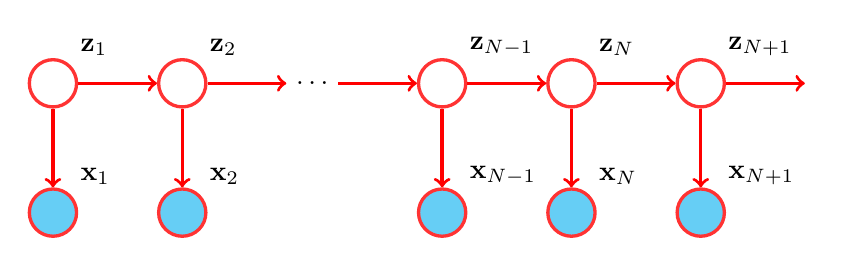
\begin{tikzpicture}[
latentnode/.style={circle, draw=red!80, minimum size=6mm, very thick},
observednode/.style={circle, draw=red!80, fill=cyan!60, minimum size=6mm, very thick},
]

% Defining the nodes
\node[latentnode, label=above right:{${\bf z}_1$}] (z1) {};
\node[latentnode, label=above right:{${\bf z}_2$}] (z2) [right=of z1] {};
\node (transition) [right=of z2] {$\ldots$};
\node[latentnode, label=above right:{${\bf z}_{N-1}$}] (z_nm1) [right=of transition] {};
\node[latentnode, label=above right:{${\bf z}_{N}$}] (zn) [right=of z_nm1] {};
\node[latentnode, label=above right:{${\bf z}_{N+1}$}] (z_np1) [right=of zn] {};
\node (final) [right=of z_np1] {};

% Defining observed nodes
\node[observednode, label=above right:{${\bf x}_1$}] (x1) [below=of z1]{};
\node[observednode, label=above right:{${\bf x}_2$}] (x2) [below=of z2]{};
\node[observednode, label=above right:{${\bf x}_{N-1}$}] (x_nm1) [below=of z_nm1]{};
\node[observednode, label=above right:{${\bf x}_{N}$}] (xn) [below=of zn]{};
\node[observednode, label=above right:{${\bf x}_{N+1}$}] (x_np1) [below=of z_np1]{};


% Relationships between latent variables
\draw[->, color=red, very thick] (z1) -- (z2);
\draw[->, color=red, very thick] (z2) -- (transition);
\draw[->, color=red, very thick] (transition) -- (z_nm1);
\draw[->, color=red, very thick] (z_nm1) -- (zn);
\draw[->, color=red, very thick] (zn) -- (z_np1);
% final node
\draw[->, color=red, very thick] (z_np1) -- (final);

% Relationships between observed and latent variables
\draw[->, color=red, very thick] (z1) -- (x1);
\draw[->, color=red, very thick] (z2) -- (x2);
\draw[->, color=red, very thick] (z_nm1) -- (x_nm1);
\draw[->, color=red, very thick] (zn) -- (xn);
\draw[->, color=red, very thick] (z_np1) -- (x_np1);

\end{tikzpicture}
	\caption{Graphical representation of a pLDS. The filled nodes represent observed variables, whereas the unfilled nodes represent latent variables.}
	\label{fig:lds-gm}
\end{figure}

The graphical representation of the Bayesian network induces the following joint distribution between latent and random variables:
\begin{equation}
	p({\bf X}, {\bf Z} \vert\boldsymbol\theta) = p(\z_1)\prod_{n=2}^N p(\z_n\vert \z_{n-1})\prod_{n=1}^N p(\x_n\vert \z_n).
\end{equation}

The graphical representation of a model not only illustrates the relationship between random variables, but it can also be used to simplify the representation of conditional probabilities using a set of rules known as \textit{d-separation}. Before we introduce the rules of $d$-separation, we define what a descendant is, and show the types of connections in a Bayesian network.

\begin{definition}
	Let $\mathcal G = \{\mathscr{N}, \mathscr{E}\}$ be a Bayesian network, and let $a \in \mathscr{N}$, $b \in \mathscr{N}$. We define a node $b$ as a \textbf{descendant} of node $a$ if there exists a path from $a$ to $b$.
\end{definition}

Let $a$, $b$, and $c$ be three nodes of a bayesian network $\mathcal G$. We say that
\begin{itemize}
	\item $a$ and $b$ meet \textbf{head-to-head} at $c$ if $a \rightarrow c \leftarrow b $;
	\item $a$ and $b$ meet \textbf{tail-to-tail} at $c$ if $a \leftarrow c \rightarrow b $;
	\item $a$ and $b$ meet \textbf{head-to-tail} at $c$ if $a \rightarrow c \rightarrow b $;
\end{itemize}

\begin{proposition}
	(\textbf{d-separation}) Let $\mathcal G = \{\{A, B, C\}, \mathscr{E}\}$ be a Bayesian network with with $A$, $B$, and $C$ arbitrary nonintersecting set of nodes. To assert whether $A \perp B \vert C$ is induced by the network, we consider all possible paths from any node in $A$ to any node in $B$. Any such path is said to be \textbf{blocked} if it includes a node such that either
	\begin{enumerate}
		\item the arrows on the path meet either head-to-tail or tail-to-tail at a node in the set $C$, or
		\item the arrows meet head-to-head at a node not in the set $C$, or any of its descendants.
	\end{enumerate}
	If all paths are blocked, then $A$ is said to be $d$-separable from $B$ by $C$, and the joint distribution over all variables in the graph satisfies $A \perp B \vert C$.
\end{proposition}

% Finally, 
% * Motivate the following proposition: It helps us decompose the conditional dependencies of the graph and simplify the computations of the E-step
% * Show the following proposition using d-separation

To exemplify the use of $d$-separation, we present the following proposition which simplifies later computations when developing the pLDS model.

\begin{proposition} \label{prop:graphical-models-separation}
	Let $({\bf Z}, {\bf X})$ be the complete-dataset of a pLDS model. Then,
	\begin{align}
		p({\bf X}\vert\z_n) &= p({\x_1, \ldots, \x_n \vert \z_n})p({\x_{n+1}, \ldots, \x_N \vert \z_n}), \label{eq:gm-1}\\
		p(\x_1, \ldots, \x_{n-1}\vert \x_n, \z_n) &= p(\x_1, \ldots, \x_{n-1}\vert \z_n), \label{eq:gm-2}\\
		p(\x_1, \ldots, \x_{n-1}\vert \z_{n-1}, \z_{n}) &= p(\x_1, \ldots, \x_{n-1}\vert \z_{n-1}), \label{eq:gm-3}\\
		p(\x_{n+1}, \ldots, \x_N \vert \z_n, \z_{n+1}) &= p(\x_{n+1}, \ldots, \x_N \vert \z_n), \label{eq:gm-4}\\
		p(\x_{n+2}, \ldots, \x_N\vert \x_{n+1}, \z_{n+1}) &= p(\x_{n+2}, \ldots, \x_N \vert \z_{n+1}),\label{eq:gm-5}\\
		p({\bf X}\vert \z_{n-1}, \z_{n}) &= p(\x_1, \ldots, \x_{n-1}\vert \z_{n-1})\cdot \nonumber\\
			&\hspace{1cm}p(\x_n\vert \z_n) p(\x_{n+1}, \ldots, \x_N \vert \z_n), \label{eq:gm-6}\\
		p(\x_{N+1} \vert {\bf X}, \z_{N+1}) &= p(\x_{N+1} \vert \z_{N+1}), \label{eq:gm-7}\\
		p(\z_{N+1} \vert {\bf X}, \z_{N}) &= p(\z_{N+1} \vert \z_{N}). \label{eq:gm-8}\\
	\end{align}
\end{proposition}

\begin{proof}
	All equations in Proposition \ref{prop:graphical-models-separation} can be explicitly shown by expanding its components and using the probability rules of sum and product. In this work, we take a visual approach and show that the factorisations hold by using $d$-separation.
	
	Assuming that none of the data in the complete-dataset is observed, the structure of the pLDS is presented in Figure \ref{fig:lds-skeleton}.
	
	\begin{figure}[h!]
		\centering
		\resizebox{\columnwidth}{!}{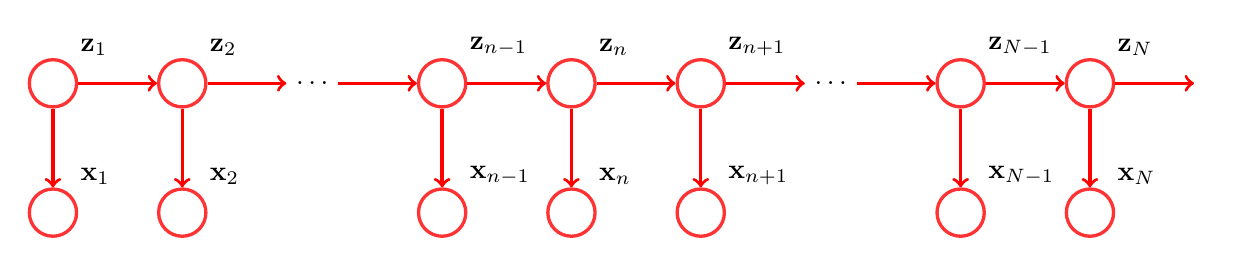
\begin{tikzpicture}[
latentnode/.style={circle, draw=red!80, minimum size=6mm, very thick},
observednode/.style={circle, draw=red!80, minimum size=6mm, very thick},
]

% Defining the nodes
\node[latentnode, label=above right:{${\bf z}_1$}] (z1) {};
\node[latentnode, label=above right:{${\bf z}_2$}] (z2) [right=of z1] {};
\node (transition) [right=of z2] {$\ldots$};
\node[latentnode, label=above right:{${\bf z}_{n-1}$}] (z_nm1) [right=of transition] {};
\node[latentnode, label=above right:{${\bf z}_{n}$}] (zn) [right=of z_nm1] {};
\node[latentnode, label=above right:{${\bf z}_{n+1}$}] (z_np1) [right=of zn] {};
\node (transition2) [right=of z_np1] {$\ldots$};
\node[latentnode, label=above right:{${\bf z}_{N-1}$}] (z_Nm1) [right=of transition2] {};
\node[latentnode, label=above right:{${\bf z}_{N}$}] (zN) [right=of z_Nm1] {};
\node (final) [right=of zN] {};

% Defining observed nodes
\node[observednode, label=above right:{${\bf x}_1$}] (x1) [below=of z1]{};
\node[observednode, label=above right:{${\bf x}_2$}] (x2) [below=of z2]{};
\node[observednode, label=above right:{${\bf x}_{n-1}$}] (x_nm1) [below=of z_nm1]{};
\node[observednode, label=above right:{${\bf x}_{n}$}] (xn) [below=of zn]{};
\node[observednode, label=above right:{${\bf x}_{n+1}$}] (x_np1) [below=of z_np1]{};
\node[observednode, label=above right:{${\bf x}_{N-1}$}] (x_Nm1) [below=of z_Nm1]{};
\node[observednode, label=above right:{${\bf x}_{N}$}] (xN) [below=of zN]{};


% Relationships between latent variables
\draw[->, color=red, very thick] (z1) -- (z2);
\draw[->, color=red, very thick] (z2) -- (transition);
\draw[->, color=red, very thick] (transition) -- (z_nm1);
\draw[->, color=red, very thick] (z_nm1) -- (zn);
\draw[->, color=red, very thick] (zn) -- (z_np1);
\draw[->, color=red, very thick] (z_np1) -- (transition2);
\draw[->, color=red, very thick] (transition2) -- (z_Nm1);
\draw[->, color=red, very thick] (z_Nm1) -- (zN);
\draw[->, color=red, very thick] (zN) -- (final);


% Relationships between observed and latent variables
\draw[->, color=red, very thick] (z1) -- (x1);
\draw[->, color=red, very thick] (z2) -- (x2);
\draw[->, color=red, very thick] (z_nm1) -- (x_nm1);
\draw[->, color=red, very thick] (zn) -- (xn);
\draw[->, color=red, very thick] (z_np1) -- (x_np1);
\draw[->, color=red, very thick] (z_Nm1) -- (x_Nm1);
\draw[->, color=red, very thick] (zN) -- (xN);

\end{tikzpicture}}
		\caption{Probabilistic structure of a pLDS.}
		\label{fig:lds-skeleton}
	\end{figure}

	We begin from equation \eqref{eq:gm-1}. The graph that induces the conditional probability $p(\X \vert \z_n)$ is given by Figure \ref{fig:gm-1}. Let $A = \{\x_1, \ldots, \x_{n-1}\}$, $B = \{x_{n+1}, \ldots, \x_N\}$, and $C = \{\z_n\}$. Notice that the connection from any node in $A$ to any node in $B$ meets head-to-tail with $C$. Hence, $A \perp B \vert C$.
	
	\begin{figure}[h!]
		\centering
		\resizebox{\columnwidth}{!}{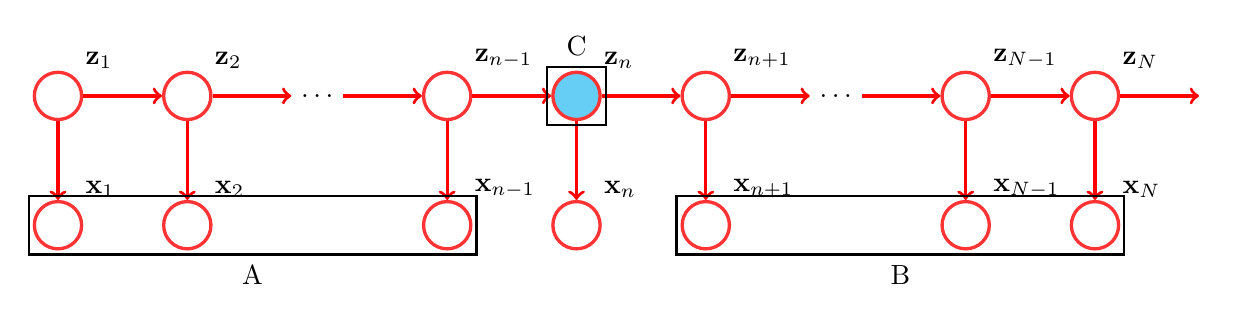
\begin{tikzpicture}[
latentnode/.style={circle, draw=red!80, minimum size=6mm, very thick},
observednode/.style={circle, draw=red!80, fill=cyan!60, minimum size=6mm, very thick},
]

% Defining the nodes
\node[latentnode, label=above right:{${\bf z}_1$}] (z1) {};
\node[latentnode, label=above right:{${\bf z}_2$}] (z2) [right=of z1] {};
\node (transition) [right=of z2] {$\ldots$};
\node[latentnode, label=above right:{${\bf z}_{n-1}$}] (z_nm1) [right=of transition] {};
\node[observednode, label=above right:{${\bf z}_{n}$}] (zn) [right=of z_nm1] {};
\node[latentnode, label=above right:{${\bf z}_{n+1}$}] (z_np1) [right=of zn] {};
\node (transition2) [right=of z_np1] {$\ldots$};
\node[latentnode, label=above right:{${\bf z}_{N-1}$}] (z_Nm1) [right=of transition2] {};
\node[latentnode, label=above right:{${\bf z}_{N}$}] (zN) [right=of z_Nm1] {};
\node (final) [right=of zN] {};

% Defining observed nodes
\node[latentnode, label=above right:{${\bf x}_1$}] (x1) [below=of z1]{};
\node[latentnode, label=above right:{${\bf x}_2$}] (x2) [below=of z2]{};
\node[latentnode, label=above right:{${\bf x}_{n-1}$}] (x_nm1) [below=of z_nm1]{};
\node[latentnode, label=above right:{${\bf x}_{n}$}] (xn) [below=of zn]{};
\node[latentnode, label=above right:{${\bf x}_{n+1}$}] (x_np1) [below=of z_np1]{};
\node[latentnode, label=above right:{${\bf x}_{N-1}$}] (x_Nm1) [below=of z_Nm1]{};
\node[latentnode, label=above right:{${\bf x}_{N}$}] (xN) [below=of zN]{};


% Relationships between latent variables
\draw[->, color=red, very thick] (z1) -- (z2);
\draw[->, color=red, very thick] (z2) -- (transition);
\draw[->, color=red, very thick] (transition) -- (z_nm1);
\draw[->, color=red, very thick] (z_nm1) -- (zn);
\draw[->, color=red, very thick] (zn) -- (z_np1);
\draw[->, color=red, very thick] (z_np1) -- (transition2);
\draw[->, color=red, very thick] (transition2) -- (z_Nm1);
\draw[->, color=red, very thick] (z_Nm1) -- (zN);
\draw[->, color=red, very thick] (zN) -- (final);


% Relationships between observed and latent variables
\draw[->, color=red, very thick] (z1) -- (x1);
\draw[->, color=red, very thick] (z2) -- (x2);
\draw[->, color=red, very thick] (z_nm1) -- (x_nm1);
\draw[->, color=red, very thick] (zn) -- (xn);
\draw[->, color=red, very thick] (z_np1) -- (x_np1);
\draw[->, color=red, very thick] (z_Nm1) -- (x_Nm1);
\draw[->, color=red, very thick] (zN) -- (xN);

\node[draw, thick, inner sep=0.5mm,label=below:A,fit=(x1) (x_nm1)] {};
\node[draw, thick, inner sep=0.5mm,label=below:B,fit=(x_np1) (xN)] {};
\node[draw, thick, inner sep=0.5mm,label=above:C,fit=(zn)] {};

\end{tikzpicture}}
		\caption{Graphical representation of equation \eqref{eq:gm-1}}
		\label{fig:gm-1}
	\end{figure}
	
	Next, we show equation \eqref{eq:gm-2}. Taking $A = \{\x_1, \ldots, \x_{n-1}\}$, $B = \{\x_n\}$, and $C = \{\z_n\}$, we observe that any node in $A$ to $\x_n$ meet head-to-tail at $\z_n$. Hence $A \perp \x_n \vert \z_n$ (see Figure \ref{fig:gm-2}). 
	\begin{figure}[h!]
		\centering
		\resizebox{\columnwidth}{!}{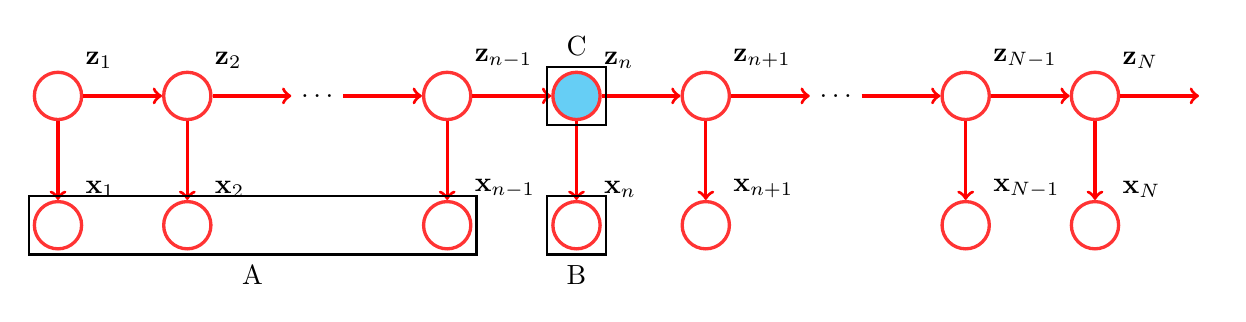
\begin{tikzpicture}[
latentnode/.style={circle, draw=red!80, minimum size=6mm, very thick},
observednode/.style={circle, draw=red!80, fill=cyan!60, minimum size=6mm, very thick},
]

% Defining the nodes
\node[latentnode, label=above right:{${\bf z}_1$}] (z1) {};
\node[latentnode, label=above right:{${\bf z}_2$}] (z2) [right=of z1] {};
\node (transition) [right=of z2] {$\ldots$};
\node[latentnode, label=above right:{${\bf z}_{n-1}$}] (z_nm1) [right=of transition] {};
\node[observednode, label=above right:{${\bf z}_{n}$}] (zn) [right=of z_nm1] {};
\node[latentnode, label=above right:{${\bf z}_{n+1}$}] (z_np1) [right=of zn] {};
\node (transition2) [right=of z_np1] {$\ldots$};
\node[latentnode, label=above right:{${\bf z}_{N-1}$}] (z_Nm1) [right=of transition2] {};
\node[latentnode, label=above right:{${\bf z}_{N}$}] (zN) [right=of z_Nm1] {};
\node (final) [right=of zN] {};

% Defining observed nodes
\node[latentnode, label=above right:{${\bf x}_1$}] (x1) [below=of z1]{};
\node[latentnode, label=above right:{${\bf x}_2$}] (x2) [below=of z2]{};
\node[latentnode, label=above right:{${\bf x}_{n-1}$}] (x_nm1) [below=of z_nm1]{};
\node[latentnode, label=above right:{${\bf x}_{n}$}] (xn) [below=of zn]{};
\node[latentnode, label=above right:{${\bf x}_{n+1}$}] (x_np1) [below=of z_np1]{};
\node[latentnode, label=above right:{${\bf x}_{N-1}$}] (x_Nm1) [below=of z_Nm1]{};
\node[latentnode, label=above right:{${\bf x}_{N}$}] (xN) [below=of zN]{};


% Relationships between latent variables
\draw[->, color=red, very thick] (z1) -- (z2);
\draw[->, color=red, very thick] (z2) -- (transition);
\draw[->, color=red, very thick] (transition) -- (z_nm1);
\draw[->, color=red, very thick] (z_nm1) -- (zn);
\draw[->, color=red, very thick] (zn) -- (z_np1);
\draw[->, color=red, very thick] (z_np1) -- (transition2);
\draw[->, color=red, very thick] (transition2) -- (z_Nm1);
\draw[->, color=red, very thick] (z_Nm1) -- (zN);
\draw[->, color=red, very thick] (zN) -- (final);


% Relationships between observed and latent variables
\draw[->, color=red, very thick] (z1) -- (x1);
\draw[->, color=red, very thick] (z2) -- (x2);
\draw[->, color=red, very thick] (z_nm1) -- (x_nm1);
\draw[->, color=red, very thick] (zn) -- (xn);
\draw[->, color=red, very thick] (z_np1) -- (x_np1);
\draw[->, color=red, very thick] (z_Nm1) -- (x_Nm1);
\draw[->, color=red, very thick] (zN) -- (xN);

\node[draw, thick, inner sep=0.5mm,label=below:A,fit=(x1) (x_nm1)] {};
\node[draw, thick, inner sep=0.5mm,label=below:B,fit=(xn)] {};
\node[draw, thick, inner sep=0.5mm,label=above:C,fit=(zn)] {};

\end{tikzpicture}}
		\caption{Graphical representation of equation \eqref{eq:gm-2}}
		\label{fig:gm-2}
	\end{figure}

	Following the same logic, we can show that equations \eqref{eq:gm-3}, \eqref{eq:gm-4}, \eqref{eq:gm-5}, \eqref{eq:gm-7}, and \eqref{eq:gm-8}  meet either head-to-tail or tail-to-tail at a node in the set $C$. We present the graphical representations of equations \eqref{eq:gm-3}, \eqref{eq:gm-4}, and \eqref{eq:gm-5} in Figures \ref{fig:gm-3}, \ref{fig:gm-4}, and \ref{fig:gm-5}.
	\begin{figure}[h!]
		\centering
		\resizebox{\columnwidth}{!}{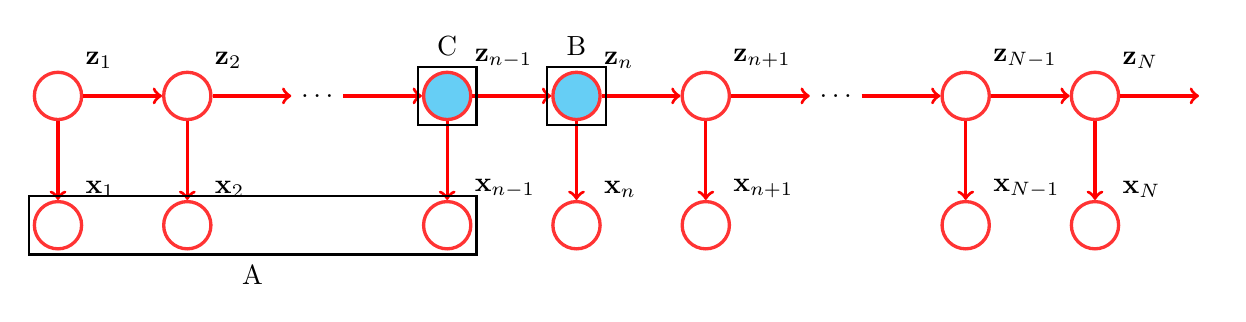
\begin{tikzpicture}[
latentnode/.style={circle, draw=red!80, minimum size=6mm, very thick},
observednode/.style={circle, draw=red!80, fill=cyan!60, minimum size=6mm, very thick},
]

% Defining the nodes
\node[latentnode, label=above right:{${\bf z}_1$}] (z1) {};
\node[latentnode, label=above right:{${\bf z}_2$}] (z2) [right=of z1] {};
\node (transition) [right=of z2] {$\ldots$};
\node[observednode, label=above right:{${\bf z}_{n-1}$}] (z_nm1) [right=of transition] {};
\node[observednode, label=above right:{${\bf z}_{n}$}] (zn) [right=of z_nm1] {};
\node[latentnode, label=above right:{${\bf z}_{n+1}$}] (z_np1) [right=of zn] {};
\node (transition2) [right=of z_np1] {$\ldots$};
\node[latentnode, label=above right:{${\bf z}_{N-1}$}] (z_Nm1) [right=of transition2] {};
\node[latentnode, label=above right:{${\bf z}_{N}$}] (zN) [right=of z_Nm1] {};
\node (final) [right=of zN] {};

% Defining observed nodes
\node[latentnode, label=above right:{${\bf x}_1$}] (x1) [below=of z1]{};
\node[latentnode, label=above right:{${\bf x}_2$}] (x2) [below=of z2]{};
\node[latentnode, label=above right:{${\bf x}_{n-1}$}] (x_nm1) [below=of z_nm1]{};
\node[latentnode, label=above right:{${\bf x}_{n}$}] (xn) [below=of zn]{};
\node[latentnode, label=above right:{${\bf x}_{n+1}$}] (x_np1) [below=of z_np1]{};
\node[latentnode, label=above right:{${\bf x}_{N-1}$}] (x_Nm1) [below=of z_Nm1]{};
\node[latentnode, label=above right:{${\bf x}_{N}$}] (xN) [below=of zN]{};


% Relationships between latent variables
\draw[->, color=red, very thick] (z1) -- (z2);
\draw[->, color=red, very thick] (z2) -- (transition);
\draw[->, color=red, very thick] (transition) -- (z_nm1);
\draw[->, color=red, very thick] (z_nm1) -- (zn);
\draw[->, color=red, very thick] (zn) -- (z_np1);
\draw[->, color=red, very thick] (z_np1) -- (transition2);
\draw[->, color=red, very thick] (transition2) -- (z_Nm1);
\draw[->, color=red, very thick] (z_Nm1) -- (zN);
\draw[->, color=red, very thick] (zN) -- (final);


% Relationships between observed and latent variables
\draw[->, color=red, very thick] (z1) -- (x1);
\draw[->, color=red, very thick] (z2) -- (x2);
\draw[->, color=red, very thick] (z_nm1) -- (x_nm1);
\draw[->, color=red, very thick] (zn) -- (xn);
\draw[->, color=red, very thick] (z_np1) -- (x_np1);
\draw[->, color=red, very thick] (z_Nm1) -- (x_Nm1);
\draw[->, color=red, very thick] (zN) -- (xN);

\node[draw, thick, inner sep=0.5mm,label=below:A,fit=(x1) (x_nm1)] {};
\node[draw, thick, inner sep=0.5mm,label=above:B,fit=(zn)] {};
\node[draw, thick, inner sep=0.5mm,label=above:C,fit=(z_nm1)] {};

\end{tikzpicture}}
		\caption{Graphical representation of equation \eqref{eq:gm-3}}
		\label{fig:gm-3}
	\end{figure}
	
	\begin{figure}[h!]
		\centering
		\resizebox{\columnwidth}{!}{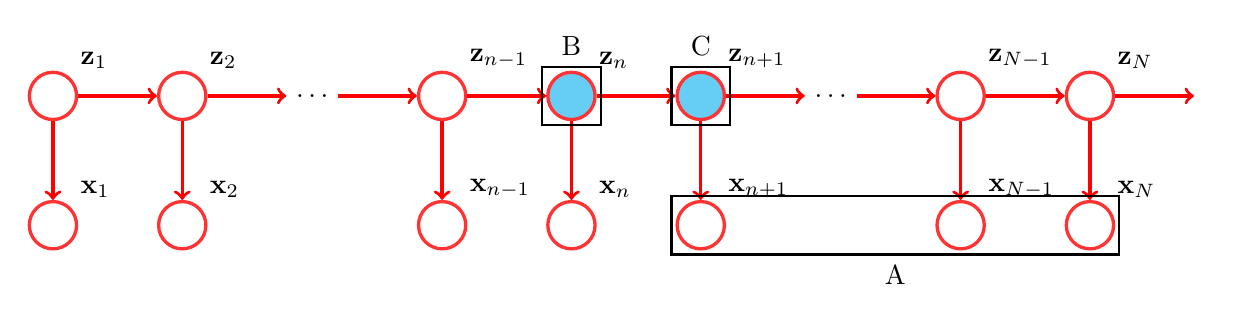
\begin{tikzpicture}[
latentnode/.style={circle, draw=red!80, minimum size=6mm, very thick},
observednode/.style={circle, draw=red!80, fill=cyan!60, minimum size=6mm, very thick},
]

% Defining the nodes
\node[latentnode, label=above right:{${\bf z}_1$}] (z1) {};
\node[latentnode, label=above right:{${\bf z}_2$}] (z2) [right=of z1] {};
\node (transition) [right=of z2] {$\ldots$};
\node[latentnode, label=above right:{${\bf z}_{n-1}$}] (z_nm1) [right=of transition] {};
\node[observednode, label=above right:{${\bf z}_{n}$}] (zn) [right=of z_nm1] {};
\node[observednode, label=above right:{${\bf z}_{n+1}$}] (z_np1) [right=of zn] {};
\node (transition2) [right=of z_np1] {$\ldots$};
\node[latentnode, label=above right:{${\bf z}_{N-1}$}] (z_Nm1) [right=of transition2] {};
\node[latentnode, label=above right:{${\bf z}_{N}$}] (zN) [right=of z_Nm1] {};
\node (final) [right=of zN] {};

% Defining observed nodes
\node[latentnode, label=above right:{${\bf x}_1$}] (x1) [below=of z1]{};
\node[latentnode, label=above right:{${\bf x}_2$}] (x2) [below=of z2]{};
\node[latentnode, label=above right:{${\bf x}_{n-1}$}] (x_nm1) [below=of z_nm1]{};
\node[latentnode, label=above right:{${\bf x}_{n}$}] (xn) [below=of zn]{};
\node[latentnode, label=above right:{${\bf x}_{n+1}$}] (x_np1) [below=of z_np1]{};
\node[latentnode, label=above right:{${\bf x}_{N-1}$}] (x_Nm1) [below=of z_Nm1]{};
\node[latentnode, label=above right:{${\bf x}_{N}$}] (xN) [below=of zN]{};


% Relationships between latent variables
\draw[->, color=red, very thick] (z1) -- (z2);
\draw[->, color=red, very thick] (z2) -- (transition);
\draw[->, color=red, very thick] (transition) -- (z_nm1);
\draw[->, color=red, very thick] (z_nm1) -- (zn);
\draw[->, color=red, very thick] (zn) -- (z_np1);
\draw[->, color=red, very thick] (z_np1) -- (transition2);
\draw[->, color=red, very thick] (transition2) -- (z_Nm1);
\draw[->, color=red, very thick] (z_Nm1) -- (zN);
\draw[->, color=red, very thick] (zN) -- (final);


% Relationships between observed and latent variables
\draw[->, color=red, very thick] (z1) -- (x1);
\draw[->, color=red, very thick] (z2) -- (x2);
\draw[->, color=red, very thick] (z_nm1) -- (x_nm1);
\draw[->, color=red, very thick] (zn) -- (xn);
\draw[->, color=red, very thick] (z_np1) -- (x_np1);
\draw[->, color=red, very thick] (z_Nm1) -- (x_Nm1);
\draw[->, color=red, very thick] (zN) -- (xN);

\node[draw, thick, inner sep=0.5mm,label=below:A,fit=(x_np1) (xN)] {};
\node[draw, thick, inner sep=0.5mm,label=above:B,fit=(zn)] {};
\node[draw, thick, inner sep=0.5mm,label=above:C,fit=(z_np1)] {};

\end{tikzpicture}}
		\caption{Graphical representation of equation \eqref{eq:gm-4}}
		\label{fig:gm-4}
	\end{figure}
	
	\begin{figure}[h!]
		\centering
		\resizebox{\columnwidth}{!}{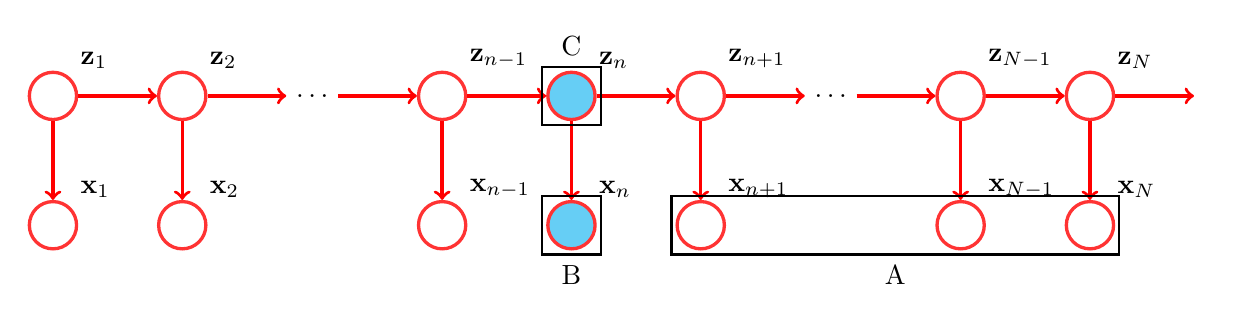
\begin{tikzpicture}[
latentnode/.style={circle, draw=red!80, minimum size=6mm, very thick},
observednode/.style={circle, draw=red!80, fill=cyan!60, minimum size=6mm, very thick},
]

% Defining the nodes
\node[latentnode, label=above right:{${\bf z}_1$}] (z1) {};
\node[latentnode, label=above right:{${\bf z}_2$}] (z2) [right=of z1] {};
\node (transition) [right=of z2] {$\ldots$};
\node[latentnode, label=above right:{${\bf z}_{n-1}$}] (z_nm1) [right=of transition] {};
\node[observednode, label=above right:{${\bf z}_{n}$}] (zn) [right=of z_nm1] {};
\node[latentnode, label=above right:{${\bf z}_{n+1}$}] (z_np1) [right=of zn] {};
\node (transition2) [right=of z_np1] {$\ldots$};
\node[latentnode, label=above right:{${\bf z}_{N-1}$}] (z_Nm1) [right=of transition2] {};
\node[latentnode, label=above right:{${\bf z}_{N}$}] (zN) [right=of z_Nm1] {};
\node (final) [right=of zN] {};

% Defining observed nodes
\node[latentnode, label=above right:{${\bf x}_1$}] (x1) [below=of z1]{};
\node[latentnode, label=above right:{${\bf x}_2$}] (x2) [below=of z2]{};
\node[latentnode, label=above right:{${\bf x}_{n-1}$}] (x_nm1) [below=of z_nm1]{};
\node[observednode, label=above right:{${\bf x}_{n}$}] (xn) [below=of zn]{};
\node[latentnode, label=above right:{${\bf x}_{n+1}$}] (x_np1) [below=of z_np1]{};
\node[latentnode, label=above right:{${\bf x}_{N-1}$}] (x_Nm1) [below=of z_Nm1]{};
\node[latentnode, label=above right:{${\bf x}_{N}$}] (xN) [below=of zN]{};


% Relationships between latent variables
\draw[->, color=red, very thick] (z1) -- (z2);
\draw[->, color=red, very thick] (z2) -- (transition);
\draw[->, color=red, very thick] (transition) -- (z_nm1);
\draw[->, color=red, very thick] (z_nm1) -- (zn);
\draw[->, color=red, very thick] (zn) -- (z_np1);
\draw[->, color=red, very thick] (z_np1) -- (transition2);
\draw[->, color=red, very thick] (transition2) -- (z_Nm1);
\draw[->, color=red, very thick] (z_Nm1) -- (zN);
\draw[->, color=red, very thick] (zN) -- (final);


% Relationships between observed and latent variables
\draw[->, color=red, very thick] (z1) -- (x1);
\draw[->, color=red, very thick] (z2) -- (x2);
\draw[->, color=red, very thick] (z_nm1) -- (x_nm1);
\draw[->, color=red, very thick] (zn) -- (xn);
\draw[->, color=red, very thick] (z_np1) -- (x_np1);
\draw[->, color=red, very thick] (z_Nm1) -- (x_Nm1);
\draw[->, color=red, very thick] (zN) -- (xN);

\node[draw, thick, inner sep=0.5mm,label=below:A,fit=(x_np1) (xN)] {};
\node[draw, thick, inner sep=0.5mm,label=below:B,fit=(xn)] {};
\node[draw, thick, inner sep=0.5mm,label=above:C,fit=(zn)] {};

\end{tikzpicture}}
		\caption{Graphical representation of equation \eqref{eq:gm-5}}
		\label{fig:gm-5}
	\end{figure}
	
	To show equation \eqref{eq:gm-6}, consider
	\begin{align}
		p(\X \vert \z_{n-1}, \z_n) &= p(\x_1, \ldots, \x_N \vert \z_{n-1},\z_n)\\
		 &= p(\x_n \vert \z_{n-1}, \z_n) p(\x_1, \ldots, \x_{n-1}, \x_{n+1}, \ldots, \x_N \vert \x_n, \z_{n-1}, \z_n)\\
		&= p(\x_n \vert \z_{n-1}, \z_n) p(\x_1, \ldots, \x_{n-1} \vert \x_n, \z_{n-1}, \z_n) \nonumber\\
			&\hspace{1cm} p(\x_{n+1}, \ldots, \x_N \vert \x_1, \ldots, \x_N, \z_{n-1}, \z_n). \label{eq:part-gm-6}
	\end{align}
	Using equation \eqref{eq:gm-2} we have $p(\x_n \vert \z_{n-1}, \z_n) = p(\x_n \vert \z_n)$. Furthermore, using equations \eqref{eq:gm-2} and \eqref{eq:gm-3}, $p(\x_1, \ldots, \x_{n-1} \vert \x_n, \z_{n-1}, \z_n) = p(\x_1, \ldots, \x_{n-1} \vert \z_{n-1})$. Finally, from equations \eqref{eq:gm-4}, and \eqref{eq:gm-5} we obtain  $p(\x_{n+1}, \ldots, \x_N \vert \x_1, \ldots, \x_N, \z_{n-1}, \z_n) = p(\x_{n+1}, \ldots, \x_N \vert  \z_{n})$. Using these results and plugging the values in \eqref{eq:part-gm-6} yields equation \eqref{eq:gm-6}.
\end{proof}


\subsection{The EM algorithm}

As we have previously mentioned, in order to find the parameters $\boldsymbol{\theta}$ that best represent the complete dataset, we maximise the log-likelihood of the complete dataset with respect to each of the parameters in $\boldsymbol{\theta}$. In this section, we present the Expectation Maximisation (EM) algorithm: a two-step iterative approach that maximises the log-likelihood of the complete-dataset. Broadly speaking, the EM algorithm is divided in two steps: the E-step attempts to estimate a plausible dataset $\Z$ given current estimates of $\boldsymbol\theta$; the M-step, fixes the estimated values of $\Z$ and updates $\boldsymbol{\theta}$. Under certain conditions, it can be shown that the EM algorithm converges to a local maximum (\cite{pml1Book}). We derive the EM algorithm in the following three propositions.

\begin{proposition} \label{prop:log-likelihood-partition}
	The log-likelihood $\log p({\bf X} \vert \boldsymbol{\theta})$ can be written as the sum of two factors
	\begin{equation}
		\log p({\bf X} \vert \boldsymbol{\theta}) = \mathcal{L}(q, \boldsymbol{\theta}) +\KL{q}{p},
	\end{equation}
	where
	\begin{align}
		\mathcal{L}(q, \boldsymbol{\theta}) &= \int q({\bf Z})\log\left(\frac{p({\bf X}, {\bf Z} \vert \boldsymbol\theta)}{q({\bf Z})}\right) d{\bf Z},\\
		\text{KL}(q \vert\vert p) &= \int q({\bf Z}) \log\left(\frac{q({\bf Z})}{p({\bf Z}\vert {\bf X}, \boldsymbol\theta)}\right) d{\bf Z}.
	\end{align}
	The term $\mathcal{L}(q, \boldsymbol\theta)$ is called the lower bound, and the term $\KL{q}{p}$ is known as the Kullback-Leibler (KL) divergence of the distributions $p$ and $q$.
\end{proposition}

\begin{proof}
	The proof follows directly from the sum of the terms $\mathcal{L}(q, \boldsymbol{\theta})$, and  $\text{KL}(q \vert\vert p)$:
	\begin{align}
		\mathcal{L}(q, \boldsymbol{\theta}) + \KL{q}{p} &= \int q({\bf Z})\log\left(\frac{p({\bf X}, {\bf Z} \vert \boldsymbol\theta)}{q({\bf Z})}\right) d{\bf Z} + \int q({\bf Z}) \log\left(\frac{q({\bf Z})}{p({\bf Z}\vert {\bf X}, \boldsymbol\theta)}\right) d{\bf Z}\\
		&= \int q({\bf Z})\left(\log p({\bf X, {\bf Z} \vert \boldsymbol{\theta}}) - \log q({\bf Z}) + \log q({\bf Z}) - \log p({\bf Z} \vert {\bf X}, \boldsymbol\theta)\right) d{\bf Z}\\
		&= \int q({\bf Z})\left(\log p({\bf X} \vert \boldsymbol{\theta}) + \log p({\bf Z} \vert {\bf X}, \boldsymbol{\theta}) - \log p({\bf Z} \vert {\bf X}, \boldsymbol\theta)\right) d{\bf Z}\\
		&= \log p({\bf X}\vert \boldsymbol\theta).
	\end{align}
	The proof also shows that maximising $\mathcal{L}(q, \boldsymbol\theta)$ increases $\log p({\bf X}\vert \boldsymbol\theta)$.
\end{proof}

The KL divergence between $p$ and $q$ serves as a nonnegative dissimilarity measure with equality to zero if and only if $q=p$  (for a proof, see \cite{pml1Book}). Hence if $q$ is a distribution intended to approximate $p$, ideally, $K(q \vert \vert p)$ should be as close to zero as possible. We note an application of the KL divergence in the following proposition.

%TODO: define a set \mathcal Q of "valid" distributions.
%TODO: why is it relevant to only maximise the lower bound L?
\begin{proposition} (\textbf{E-step})
	The function $q({\bf Z})$ that maximises the lower bound $\mathcal L(q, \boldsymbol{\theta}$) is given by
	\begin{equation}
		q(\Z) = \argmax{\hat q} \mathcal{L}(\hat q, \boldsymbol\theta) = p({\bf Z} \vert {\bf X}, \boldsymbol\theta).
	\end{equation}
\end{proposition}

\begin{proof}
	We begin by rewriting the lower bound, we obtain
	\begin{align}
		\mathcal{L}(q, \boldsymbol\theta) &= \int q(\Z)\log\left(\frac{p(\X, \Z \vert \boldsymbol\theta)}{q(\Z)}\right) d{\bf Z}\\
		&= \int q(\Z) \left(\log p(\X\vert\boldsymbol\theta) + \log\left( \frac{p(\Z \vert \X, \boldsymbol\theta)}{q(\Z)} \right) \right) d\Z\\
		&= \log p(\X \vert \boldsymbol{\theta}) - \int q(\Z) \log\left(\frac{q(\Z)}{p(\Z \vert \X, \boldsymbol\theta)}\right) d\Z\\
		&= \log p(\X \vert \boldsymbol\theta) - \KL{q}{p}. \label{eq:part-L-rewrite}
	\end{align}
	
	To find the function $q$ that maximises \eqref{eq:part-L-rewrite}, we notice that the first term does not depend on $q$. Furthermore, we observe that the second term is the negative Kullback-Leibler divergence between $q$ and $p$. Therefore, the function $q(\Z)$ that maximises the lower bound is given by $p(\Z \vert \X, \boldsymbol\theta)$.
\end{proof}

\begin{proposition}\label{prop:m-step}
	(\textbf{M-step}) Maximising $\mathcal{L}(q, \boldsymbol{\theta})$ over $\boldsymbol{\theta}$ at fixed $q({\bf Z}) = p({\bf Z} \vert {\bf X}, \boldsymbol\theta^\text{old})$ is equivalent to maximising the function
	\begin{equation}
		Q(\boldsymbol{\theta}, \boldsymbol{\theta}^\text{old}) = \mathbb{E}_{{\bf Z}\vert {\bf X}, \boldsymbol{\theta}^\text{old}}[\log p({\bf X}, {\bf Z}\vert \boldsymbol\theta)].
	\end{equation}
\end{proposition}

\begin{proof}
	We rewrite the maximisation of the lower bound with fixed $q$, and we obtain
	\begin{align}
		\boldsymbol{\theta}^\text{new} &= \argmax{\boldsymbol\theta} \mathcal{L}(q, \boldsymbol\theta)\\
		&= \argmax{\boldsymbol{\theta}} \int p(\Z \vert \X, \boldsymbol{\theta}^\text{old}) \log\left(\frac{p(\X, \Z \vert \boldsymbol\theta)}{p(\Z \vert \X, \boldsymbol\theta^\text{old})}\right) d\Z\\
		&= \argmax{\boldsymbol{\theta}} \int p(\Z \vert \X, \boldsymbol{\theta} ^\text{old}) \log p(\X, \Z \vert \boldsymbol\theta) d\Z - \int p(\Z \vert \X, \boldsymbol{\theta}^\text{old}) \log p(\Z \vert \X, \boldsymbol{\theta}^\text{old})\\
		&= \argmax{\boldsymbol{\theta}} \mathbb{E}_{{\bf Z}\vert {\bf X}, \boldsymbol{\theta}^\text{old}}[\log p({\bf X}, {\bf Z}\vert \boldsymbol\theta)].
	\end{align}
\end{proof}

The E and M steps are applied iteratively in sequence, until convergence of $\boldsymbol{\theta}$, that is, changes in theta are below a fixed tolerance.

% TODO: the EM algorithm converges under some conditions which our LDS model
% has. Write

\section{Deriving a model for the pLDS}
In this section, we derive the E-step and the M-steps for the linear dynamical system presented in the previous section.

\subsection{The E-step} \label{subsec:e-step}
To make use of the E-step, it is helpful to distinguish which elements depend on $\z_n$. Consider

\begin{align}
	\log p({\bf X}, {\bf Z}\vert \boldsymbol\theta) &= \log p(\z_1) + \sum_{n=2}^N \log p(\z_n\vert \z_{n-1}) + \sum_{n=1}^N \log p(\x_n\vert \z_n)\\
	   &=\frac{1}{2}\log\vert{\bf V}_0^{-1}\vert - \frac{1}{2}(\z_1 - \boldsymbol\mu_0)^T{\bf V}_0^{-1}(\z_1 - \boldsymbol\mu_0) \nonumber \\
	   &\hspace{1cm}+ \sum_{n=2}^N \frac{1}{2}\log\vert\boldsymbol\Gamma^{-1}\vert - \frac{1}{2}(\z_n - {\bf A z}_{n-1})^T\boldsymbol{\Gamma}^{-1}(\z_n - {\bf A z}_{n-1}) \nonumber \\
	   &\hspace{1cm}+\sum_{n=1}^N \frac{1}{2}\log\vert\boldsymbol\Sigma\vert -\frac{1}{2}(\x_n - {\bf C z}_n)^T \boldsymbol{\Sigma}^{-1}(\x_n - {\bf C z}_n) + \text{const.}\\
	   &= \frac{1}{2}\log \vert
	  {\bf V}_0^{-1}\vert -\frac{1}{2}\left[\text{Tr}\left(\z_1 \z_1^T {\bf V}_0^{-1}\right) -2 \z_1^T{\bf V}_0^{-1}\boldsymbol\mu_0 + \boldsymbol\mu_0^T {\bf V}_0^{-1}\boldsymbol\mu_0\right] \nonumber \\
	  &\hspace{1cm}+ \frac{N-1}{2}\log\vert\boldsymbol\Gamma^{-1}\vert + \frac{N}{2}\log\vert \boldsymbol\Sigma^{-1}\vert \nonumber \\
	  &\hspace{1cm}-\frac{1}{2} \sum_{n=2}^{N}\text{Tr}\big(\z_n\z_n^T\boldsymbol\Gamma^{-1} -{\bf A} \z_{n-1}\z_n^T\boldsymbol\Gamma^{-1} - \nonumber\\
	  &\hspace{1.8cm}{\bf A}^T\boldsymbol{\Gamma}^{-1}\z_n\z_{n-1}^T + {\bf A}^T \boldsymbol\Gamma^{-1}{\bf A}\z_{n-1}\z_{n-1}^T\big) \nonumber\\
	  &\hspace{1cm}-\frac{1}{2}\sum_{n=1}^N\big[\x_n^T\boldsymbol{\Sigma}^{-1}\x_n - \z_n^T{\bf C}^T\boldsymbol\Sigma^{-1}\x_n - \x_n^T\boldsymbol{\Sigma}^{-1}{\bf C}\z_n  \\
	  &\hspace{1cm} + \text{Tr}(\z_n\z_n^T{\bf C}^T\boldsymbol\Sigma^{-1}{\bf C})\big] + \text{const.}, \label{eq:complete-log-likelihood}
\end{align}

where ``const.'' denotes the terms that do not depend on $\boldsymbol{\theta}$. From equation \eqref{eq:complete-log-likelihood}, we observe that the expectation with respect to the posterior distribution is completely determined by the expectations $\mathbb{E}[\z_n]$, $\mathbb{E}[\z_n\z_{n}^{T}]$, and  $\mathbb{E}[\z_n\z_{n-1}^{T}]$. Thus, we obtain

\begin{align}
	Q(\boldsymbol\theta, \boldsymbol\theta^\text{old}) &= \frac{1}{2}\log \vert
	  {\bf V}_0^{-1}\vert -\frac{1}{2}\left[\text{Tr}\left(\mathbb{E}\left[\z_1 \z_1^T\right] {\bf V}_0^{-1}\right) -2 \mathbb{E}\left[\z_1\right]^T{\bf V}_0^{-1}\boldsymbol\mu_0 + \boldsymbol\mu_0^T {\bf V}_0^{-1}\boldsymbol\mu_0\right] \nonumber \\
	  &\hspace{1cm}+ \frac{N-1}{2}\log\vert\boldsymbol\Gamma^{-1}\vert + \frac{N}{2}\log\vert \boldsymbol\Sigma^{-1}\vert \nonumber \\
	  &\hspace{1cm}-\frac{1}{2} \sum_{n=2}^{N}\text{Tr}\big(\expectation{\z_n\z_n^T}\boldsymbol\Gamma^{-1} - {\bf A}\expectation{\z_{n-1}\z_n^T}\boldsymbol\Gamma^{-1} \nonumber\\
	  &\hspace{1.8cm} - {\bf A}^T\boldsymbol{\Gamma}^{-1}\expectation{\z_n\z_{n-1}^T} + {\bf A}^T\boldsymbol\Gamma^{-1}{\bf A}\expectation{\z_{n-1}\z_{n-1}^T}\big) \nonumber\\
	  &\hspace{1cm}-\frac{1}{2}\sum_{n=1}^N\big[\x_n^T\boldsymbol{\Sigma}^{-1}\x_n-\expectation{\z_n^T}{\bf C}^T \boldsymbol\Sigma^{-1}\x_n - \x_n^T\boldsymbol\Sigma^{-1}{\bf C}\expectation{\z_n} \nonumber\\
	  &\hspace{1cm} + \text{Tr}(\mathbb{E}\left[\z_n\z_n^T\right]{\bf C}^T\boldsymbol\Sigma^{-1}{\bf C})\big] + \text{const.}  \label{eq:Q-LDS}
\end{align}


To compute the expected values of the latent variables, we first find the posterior distribution of the latent variables $\gamma(\z_n) := p(\z_n\vert {\bf X})$, and $\xi(\z_{n-1}, \z_{n}) := p(\z_{n-1}, \z_n\vert {\bf X})$.

%why is it useful?

\begin{proposition}\label{prop:gamma-factorisation}
	The term $\gamma(\z_n)$ can be written as the product of the joint probability of the first $n$ observations $\{\x_j\}_{j=1}^n$ and $\z_n$, and the conditional probability of the observations that follow $\z_n$, i.e. $\{\x_j\}_{j=n+1}^{N}$, conditional on $\z_n$.
\end{proposition}

\begin{proof}
Denote $\alpha(\z_n) := p(\x_1, \ldots, \x_n, \z_n)$ as the joint probability of the observed data up to $n$, and $\beta(\z_n) := p(\x_{n+1}, \ldots, \x_N\vert \z_n)$ as the probability of all data that follows the $n$-th observation, conditional on the $n$-th latent variable $\z_n$. Then, consider  $\gamma(\z_n)$ and equation \eqref{eq:gm-1} from Proposition \ref{prop:graphical-models-separation}, we have
\begin{align}
	\gamma(\z_n) &= p(\z_n \vert {\bf X})\\
					  &= \frac{1}{p(\x)}p(\z_n)p({\bf X} \vert \z_n)\\
					  &= \frac{1}{p(\x)} p(\z_n) p(\x_1, \ldots, \x_n\vert \z_n) p(\x_{n+1}, \ldots, \x_N\vert \z_n) \label{eq:gamma-part-1}\\
					  &= \frac{1}{p(\x)}p(\x_1, \ldots, \x_n, \z_n) p(\x_{n+1}, \ldots, \x_N\vert \z_n)\\
					  &= \frac{1}{p(\x)}\alpha(\z_n)\beta(\z_n).
\end{align}
\end{proof}

The result in Proposition \ref{prop:gamma-factorisation} is generally applicable, but in this work we consider the case where each random variable is normally-distributed.

% Here we show that the xi can also be written in terms of alpha and beta
\begin{proposition}\label{prop:xi-factorisation}
	The term $\xi(\z_{n-1}, \z_n)$ can be written in terms of $\alpha({\cdot})$, and $\beta(\cdot)$.
\end{proposition}

\begin{proof}
	Based on the definition of $\xi(\z_{n-1}, \z_{n})$, we have
	\begin{align}
		\xi(\z_{n-1}, \z_{n}) &= p(\z_{n-1}, \z_{n} \vert \X)\\
		&= \frac{1}{p(\x)}p(\z_{n-1}, \z_{n}) p(\X \vert \z_{n-1}, \z_{n})\\
		&= \frac{1}{p(\x)} p(\z_{n-1}) p(\z_{n} \vert \z_{n-1}) p(\x_1, \ldots, \x_{n-1}\vert \z_{n-1}) \nonumber \\
			&\hspace{1cm} p(\x_n\vert \z_n) p(\x_{n+1}, \ldots, \x_N \vert \z_n) \label{eq:xi-part-1}\\
		&= \frac{1}{p(\x)} p(\z_{n} \vert \z_{n-1}) p(\x_1, \ldots, \x_{n-1}, \z_{n-1}) \nonumber \\
			&\hspace{1cm} p(\x_n\vert \z_n) p(\x_{n+1}, \ldots, \x_N \vert \z_n)\\
		&= \frac{1}{p(\x)} \alpha(\z_{n-1}) p(\z_{n} \vert \z_{n-1}) p(\x_n \vert \z_n) \beta(\z_n),
	\end{align}
where we employ equation \eqref{eq:gm-5} to derive equation \eqref{eq:xi-part-1}.
\end{proof}


% Hence, to make sense of gamma and xi we only need to find values of alpha and beta
Propositions \ref{prop:gamma-factorisation}, and \ref{prop:xi-factorisation} show that both $\gamma$ and $\xi$ are completely determined by the values of $\alpha$ and $\beta$. Hence, we only need to compute the set of values $\{\alpha(\z_n)\}_n$ and $\{\beta(\z_n)\}_n$ once per E-iteration to find the values of $\gamma$ and $\xi$. Our next step is to derive an algorithm to efficiently compute $\alpha(\z_n)$, and $\beta(\z_n)$ for every $n$.

%TODO: comment on the initial value z_1

% 	* We show that alpha can be represented as a recursive formula
\begin{proposition} \label{prop:alpha-recursive}
	$\alpha(\z_n)$ can be written recursively as
	\begin{equation}
		\alpha(\z_n) = p(\x_n\vert \z_n) \int \alpha(\z_{n-1})p(\z_n\vert\z_{n-1}) d\z_{n-1}.
	\end{equation}
\end{proposition}

\begin{proof}
	The proof follows from the definition of $\alpha(\z_n)$ and Proposition \ref{prop:graphical-models-separation}:
	\begin{align}
		\alpha(\z_n) &= p(\x_1, \ldots, \x_n, \z_n) \\
		&= p(\z_n) p(\x_1, \ldots, \x_n \vert \z_n) \\
		&= p(\z_n) p(\x_n \vert \z_n) p(\x_1, \ldots, \x_{n-1} \vert \x_n, \z_n) \\
		&= p(\z_n) p(\x_n \vert \z_n) p(\x_1, \ldots, \x_{n-1} \vert \z_n) \label{eq:alpha-part-1}\\
		&= p(\x_n \vert \z_n) p(\x_1, \ldots, \x_{n-1}, \z_n) \\
		&= p(\x_n \vert \z_n) \int p(\x_1, \ldots, \x_{n-1}, \z_{n-1}, \z_n) d\z_{n-1}\\
		&= p(\x_n \vert \z_n) \int p(\z_{n-1})p(\z_n \vert \z_{n-1})p(\x_1, \ldots, \x_{n-1} \vert \z_{n-1}, \z_n) d\z_{n-1}\\
		&= p(\x_n \vert \z_n) \int p(\z_{n-1})p(\z_n \vert \z_{n-1})p(\x_1, \ldots, \x_{n-1} \vert \z_{n-1}) d\z_{n-1} \label{eq:alpha-part-2}\\ 
		&= p(\x_n \vert \z_n) \int p(\z_n \vert \z_{n-1})p(\x_1, \ldots, \x_{n-1}, \z_{n-1}) d\z_{n-1}\\
		&= p(\x_n \vert \z_n) \int p(\z_n \vert \z_{n-1})\alpha(\z_{n-1}) d\z_{n-1},
	\end{align}
	where equation \eqref{eq:alpha-part-1} follows from equation \eqref{eq:gm-2}, and equation \eqref{eq:alpha-part-2} follows from equation \eqref{eq:gm-3}.
\end{proof}

%  	* We show that beta can be represented as a recursive formula
\begin{proposition} \label{prop:beta-recursive}
	$\beta(\z_n)$ can be written recursively as
	\begin{equation}
		\beta(\z_n) = \int  \beta(\z_{n+1})p(\x_{n+1}\vert \z_{n+1}) p(\z_{n+1}\vert \z_n) d\z_{n+1}.
	\end{equation} 
\end{proposition}

\begin{proof}
	Similarly to Proposition \ref{prop:alpha-recursive}, we show it by using the definition of $\beta(\z_n)$ and Proposition \ref{prop:graphical-models-separation}:
	\begin{align}
		\beta(\z_n) &= p(\x_{n+1}, \ldots, \x_N \vert \z_n)\\
		&= \int p(\x_{n+1}, \ldots, \x_N, \z_{n+1} \vert \z_n) d\z_{n+1} \\
		&= \int p(\z_n \vert \z_{n+1}) p(\x_{n+1}, \ldots, \x_N \vert \z_{n+1}, \z_n) d\z_{n+1} \\
		&= \int p(\z_n \vert \z_{n+1}) p(\x_{n+1}, \ldots, \x_N \vert \z_{n+1}) d\z_{n+1} \label{eq:beta-part-1} \\
		&= \int p(\z_n \vert \z_{n+1}) p(\x_{n+1} \vert \z_{n+1}) p(\x_{n+2}, \ldots, \x_N \vert \x_{n+1}, \z_{n+1}) d\z_{n+1} \\
		&= \int p(\z_n \vert \z_{n+1}) p(\x_{n+1} \vert \z_{n+1}) p(\x_{n+2}, \ldots, \x_N \vert \z_{n+1}) d\z_{n+1} \label{eq:beta-part-2}\\
		&= \int p(\z_n \vert \z_{n+1}) \beta(\z_{n+1}) d\z_{n+1},
	\end{align}
	where we derive equations \eqref{eq:beta-part-1} and \eqref{eq:beta-part-2} from equations \eqref{eq:gm-4} and \eqref{eq:gm-5}, respectively.
\end{proof}

% We argue that alpha and beta values can become small very quick, so we require another way to compute its values
For moderately large $N$, $\alpha$ and $\beta$ become small very quickly. To solve this drawback, we work with re-scaled values of $\alpha$ and $\beta$. This has the additional benefit that the re-scaled values $\alpha(\z_n)$ can be written in form of a Normal distribution whose updating equations are  called the \textbf{Kalman filter equations}. An alternative way to control for numerical underflow is to work with logarithms of probabilities. However, we will not be considering that approach in this work.

% Introduce alpha hat and beta hat: show that they can be written

\begin{proposition} \label{prop:alpha-hat}
	Defining the scaled value $\hat\alpha(\z_n)$ as
	\begin{equation}
		\hat\alpha(\z_n) := \frac{\alpha(\z_n)}{p(\x_1, \ldots, \x_n)} = p(\z_n \vert \x_1, \ldots, \x_n),
	\end{equation}
	the updating equation can be written as
	\begin{equation}
		 c_n \hat\alpha(\z_n) = p(\x_n\vert\z_n)\int \hat\alpha(\z_{n-1})p(\z_n \vert \z_{n-1}) d\z_{n-1},
	\end{equation}
	with
	\begin{equation}
		c_n = p(\x_n \vert \x_{n-1}, \ldots, \x_1),
	\end{equation}
	and
	\begin{equation}
		p(\x_1, \ldots, \x_n) = \int \alpha(\z_n) d\z_n.\\
	\end{equation}
\end{proposition}

\begin{proof}
	We define the coefficient $c_n = p(\x_n \vert \x_{n-1}, \ldots, \x_1)$ and we show
	\begin{align}
		p(\x_1, \ldots, \x_N) &=  p(\x_1) p(\x_2 \vert \x_1) \cdots p(\x_N \vert \x_1, \ldots, \x_{N-1})\\
		&= \prod_{n=1}^N c_n.
	\end{align}
	Consider the definition of $\hat\alpha(\z_n)$, we rewrite $\alpha(\z_n)$ as follows
	\begin{equation} \label{eq:alpha-rewrite}
		\alpha(\z_n) = \hat\alpha(\z_n) p(\x_1, \ldots, \x_n) = \hat\alpha(\z_n) \prod_{j=1}^n c_j.
	\end{equation}
	Using Proposition \ref{prop:alpha-recursive} and equation \eqref{eq:alpha-rewrite} we observe
	\begin{align}
		&\alpha(\z_n) = p(\x_n\vert \z_n) \int  \alpha(\z_{n-1})p(\z_n\vert\z_{n-1}) d\z_{n-1}\\
		\iff & \hat\alpha(\z_n) \prod_{j=1}^{n} c_n = p(\x_n \vert \z_n) \int  \hat\alpha(\z_{n-1}) \prod_{j=1}^{n-1} c_j \cdot  p(\z_n\vert\z_{n-1}) d\z_{n-1}\\
		\iff & \hat\alpha(\z_n) c_n =   p(\x_n \vert \z_n) \int  \hat\alpha(\z_{n-1})   p(\z_n\vert\z_{n-1}) d\z_{n-1}.
	\end{align}
\end{proof}

\begin{proposition} \label{prop:beta-hat}
	Defining the scaled value $\hat\beta(\z_n)$ as
	\begin{equation}
		\hat\beta(\z_n) = \frac{p(\x_{n+1}, \ldots, \x_N \vert \z_n)}{p(\x_{n+1}, \ldots, \x_N \vert \x_1, \ldots \x_n)},
	\end{equation}
	the updating equation can be represented as
	\begin{equation}
		\hat\beta(\z_n) = \frac{1}{c_{n+1}}\int \hat\beta(\z_{n+1})p(\x_{n+1}\vert\z_{n+1})p(\z_{n+1}\vert\z_n) d\z_{n+1},
	\end{equation}
	with
	\begin{align}
		p(\x_{n+1}, \ldots, \x_N \vert \x_1, \ldots \x_n) &= \int p(\x_{n+1}, \ldots, \x_N, \z_n \vert \x_1, \ldots \x_n) d\z_n\\
		&= \int p(\z_n \vert \x_1, \ldots \x_n) p(\x_{n+1}, \ldots, \x_N \vert \x_1, \ldots \x_n, \z_n) d\z_n \nonumber\\
		&= \int p(\z_n \vert \x_1, \ldots \x_n) p(\x_{n+1}, \ldots, \x_N \vert \z_n) d\z_n\\
		&= \frac{1}{\int \alpha(\z_n) d\z_n} \int \alpha(\z_n) \beta(\z_n) d\z_n.
	\end{align}
\end{proposition}

\begin{proof}
	We rewrite $\beta(\z_n)$ in terms of $\hat\beta(\z_n)$, and $c_n$, and we obtain
	\begin{align}
		\beta(\z_n) &= p(\x_{n+1}, \ldots, \x_N \vert \z_n)\\
		&= p(\x_{n+1}, \ldots, \x_N \vert \z_n) \frac{p(\x_{n+1}, \ldots, \x_N \vert \x_1, \ldots \x_n)}{p(\x_{n+1}, \ldots, \x_N \vert \x_1, \ldots \x_n)} \\
		&= p(\x_{n+1}, \ldots, \x_N \vert \x_1, \ldots \x_n) \frac{p(\x_{n+1}, \ldots, \x_N \vert \z_N)}{p(\x_{n+1}, \ldots, \x_N \vert \x_1, \ldots \x_n)}\\
		&= p(\x_{n+1}, \ldots, \x_N \vert \x_1, \ldots \x_n) \hat\beta(\z_n)\\
		&= \hat\beta(\z_n) p(\x_{n+1} \vert \x_1, \ldots \x_n) \cdot \ldots \cdot p(\x_{N} \vert \x_1, \ldots \x_{N-1})\\
		&= \hat\beta(\z_n) \prod_{j=n+1}^N c_j \label{eq:beta-rewrite}.
	\end{align}
	Using Proposition \ref{prop:beta-recursive} and equation \eqref{eq:beta-rewrite}, we obtain
	\begin{align}
		&\beta(\z_n) = \int  \beta(\z_{n+1})p(\x_{n+1}\vert \z_{n+1}) p(\z_{n+1}\vert \z_n) d\z_{n+1}\\
		\iff& \hat\beta(\z_n) \prod_{j=n+1}^N c_j = \int \hat\beta(\z_{n+1}) \prod_{j=n+2}^N c_jp(\x_{n+1}\vert \z_{n+1}) p(\z_{n+1}\vert \z_n) d\z_{n+1}\\
		\iff& c_{n+1} \hat\beta(\z_n) = \int  \hat\beta(\z_{n+1}) p(\x_{n+1}\vert \z_{n+1}) p(\z_{n+1}\vert \z_n) d\z_{n+1}.
	\end{align}
\end{proof}

%% Proposition is never used (?) Check
%\begin{proposition}
%	The term $c_n$ can be written as a recursive term of the form
%	\begin{equation}
%		c_n = \int_{\z_n} p(\x_n \vert \z_n) \int  \hat\alpha(\z_{n-1})p(\z_n \vert \z_{n-1}) d\z_n\z_{n-1}.
%	\end{equation}
%\end{proposition}
%
%\begin{proof}
%	\texttt{TODO: write proof}
%\end{proof}

The term $\hat\alpha(\z_n)$ is called the $\alpha$-forward message passing for a linear dynamical system or \textbf{Kalman filter equation}.  The term $\hat\beta(\z_n)$ is called the $\beta$-backward message passing of a linear dynamical system or \textbf{Kalman smoother equation}. Intuitively, $\hat\alpha(\z_n)$ represents the information that the history of the data has on the $n$-th latent state, whereas $\hat\beta(\z_n)$ represents how a latent variable with known value at time $n$ affects the future behaviour of the system.

In the following two propositions we show that $\gamma(\z_n)$ and $\xi(\z_{n-1}, \z_{n})$ can be written in terms of $\hat\alpha$ and $\hat\beta$. We later show that this induces a normal probability density function for $\gamma(\z_n)$ in terms of a recursive formula that allows to efficiently compute the expected values $\mathbb{E}[\z_n]$, $\mathbb{E}[\z_n\z_{n}^{T}]$, and  $\mathbb{E}[\z_n\z_{n-1}^{T}]$.

% Show that gamma and xi can be written in terms of \hat\alpha and \hat\beta.

\begin{proposition}\label{prop:gamma-rewrite-scaled}
	The term $\gamma(\z_n)$ can be written in terms of the re-scaled factors $\hat\alpha(\z_n)$, and $\hat\beta(\z_n)$ as
	\begin{equation}
		\gamma(\z_n) = \hat\alpha(\z_n)\hat\beta(\z_n).
	\end{equation}
\end{proposition}

\begin{proof} We write down the definition for $\gamma(\z_n)$ and considering equations \eqref{eq:alpha-rewrite}, and \eqref{eq:beta-rewrite}, we obtain
	\begin{align}
		\gamma(\z_n) &= \frac{\alpha(\z_n) \beta(\z_n)}{p({\bf X})} \\
		&= \frac{1}{p({\bf X})}\left(\hat\alpha(\z_n) \prod_{j=1}^n c_j\right)\left(\hat\beta(\z_n) \prod_{j={n+1}}^N c_j\right) \\
		&= \frac{1}{p(\bf X)} \prod_{j=1}^N c_j \cdot \hat\alpha(\z_n) \hat\beta(\z_n)\\
		&= \hat\alpha(\z_n) \hat\beta(\z_n).
	\end{align}
\end{proof}

\begin{proposition} \label{prop:xi-rewrite}
	$\xi(\z_{n-1}, \z_n)$ can be written in terms of the re-scaled factors $\hat\alpha(\z_n)$ and $\hat\beta(\z_n)$ as
	\begin{equation}
		\xi(\z_{n-1}, \z_{n}) = c_n^{-1}\hat\alpha(\z_n)p(\x_n \vert \z_n) p(\z_{n-1}\vert \z_n)\hat\beta(\z_n).
	\end{equation}
\end{proposition}

\begin{proof}
	\begin{align}
		\xi(\z_{n-1}, \z_n) &= \frac{1}{p({\bf X})} \alpha(\z_n) p(\x_n \vert \z_n) p(\z_{n-1} \vert \z_n) \beta(\z_n) \\
		&= \left(\prod_{j=1}^N c_j\right)^{-1} \left(\hat\alpha(\z_{n-1}) \prod_{j=1}^{n-1} c_j\right)p(\x_n \vert \z_n) p(\z_{n-1} \vert \z_n)\left(\hat\beta(\z_n) \prod_{j={n+1}}^N c_j\right) \\
		&= \left(\prod_{j=1}^N c_j\right)^{-1} \left(\prod_{j\neq n}^N c_j\right) \hat\alpha(\z_{n-1}) p(\x_n \vert \z_n) p(\z_{n-1} \vert \z_n) \hat\beta(\z_n)\\
		&= c_n^{-1}\hat\alpha(\z_{n-1}) p(\x_n \vert \z_n) p(\z_{n-1} \vert \z_n) \hat\beta(\z_n).
	\end{align}
\end{proof}

As we have previously mentioned, the term $\hat\alpha(\z_n)$ can be represented as the probability density function of a normal distribution whose mean and covariance matrix depend on previous means and covariances. We formalise this in the following two theorems

% TODO: write it more clearly
% Show that alpha hat is a normal distribution
%	* Derive the Kalman Filter Equations
\begin{theorem} (\textbf{Kalman Filter: initial condition}) \label{theorem:kalman-filter-initial}
	The factor $\hat\alpha(\z_1)$ can be written as a normal probability density function with mean and covariance matrix given by
	\begin{align}
		\boldsymbol{\mu}_1 &= \boldsymbol{\mu}_0 + {\bf K}_1(\x_1 -{\bf C}\boldsymbol\mu_0),\\
		{\bf V}_1 &=  ({\bf I} - {\bf K}_1{\bf C}){\bf V}_0.
	\end{align}
	Furthermore, $c_1$ is a normal probability density function of the form
	\begin{equation}
		c_1 = \N(\x_1\vert {\bf C}\boldsymbol\mu_0, \boldsymbol\Sigma + {\bf C} {\bf V}_0 {\bf C}),
	\end{equation}
	with ${\bf K}_1 = {\bf V}_0{\bf C}^T({\bf C} {\bf V}_0 {\bf C}^T + \boldsymbol\Sigma)^{-1}$.
\end{theorem}

\begin{proof}
	From Proposition \ref{prop:alpha-hat} we have $\hat\alpha(\z_1) = p(\z_1\vert\x_1)$. Then, $\hat\alpha(\z_1) \propto p(\z_1)p(\x_1\vert\z_1) = \N(\z_1 \vert \boldsymbol\mu_0, {\bf V}_0) \N(\x_1\vert {\bf C}\z_1, \boldsymbol\Sigma)$. Thus, $\hat\alpha(\z_1)$ is a Normal distribution with mean $\boldsymbol{\mu}_1$ and covariance matrix ${\bf V}_1$. We write
	\begin{align}
		&c_1 \hat\alpha(\z_1) = \N(\z_1 \vert \boldsymbol\mu_0, {\bf V}_0) \N(\x_1\vert {\bf C}\z_1, \boldsymbol\Sigma)\\
		\iff& c_1 \N(\z_1\vert \boldsymbol\mu, {\bf V}_1) = \N(\z_1 \vert \boldsymbol\mu_0, {\bf V}_0) \N(\x_1\vert {\bf C}\z_1, \boldsymbol\Sigma),
	\end{align}
	where $c_1$ is the normalisation coefficient. To find $\boldsymbol{\mu}_1$ and ${\bf V}_1$, we make use of equation \eqref{eq:normal-conditional} to obtain
	\begin{align}
		\boldsymbol{\mu}_1 &= \left({\bf V}_0^{-1} + {\bf C}^T\boldsymbol{\Sigma}^{-1} {\bf C}\right)^{-1} \left\{{\bf C}\boldsymbol\Sigma^{-1}\x_1 + {\bf V}_0^{-1}\boldsymbol\mu_0\right\},\\
		{\bf V}_1 &= \left({\bf V}_0^{-1} + {\bf C}^T\boldsymbol{\Sigma}^{-1} {\bf C}\right)^{-1}.
	\end{align}
	Then, we rewrite the covariance matrix using Proposition \ref{prop:woodbury-identity} as
	\begin{align}
		{\bf V}_1 &= \left({\bf V}_0^{-1} + {\bf C}^T\boldsymbol{\Sigma}^{-1} {\bf C}\right)^{-1}\\
		&= {\bf V}_0 - {\bf V}_0 {\bf C}^T\left(\boldsymbol\Sigma + {\bf C}{\bf V}_0{\bf C}^T\right)^{-1}{\bf C}{\bf V}_0 \\
		&= {\bf V}_0 - {\bf K}_1{\bf C}{\bf V}_0\\
		&= ({\bf I} - {\bf K}_1{\bf C}){\bf V}_0, \label{eq:part-v1-rewrite}
	\end{align}
	where we have defined ${\bf K}_1 := {\bf V}_0 {\bf C}^T\left(\boldsymbol\Sigma + {\bf C}{\bf V}_0{\bf C}^T\right)^{-1}$. The result derived in Proposition \ref{prop:matrix-rewrite1} allows us to rewrite ${\bf K}_1$ as follows
	\begin{align}
		{\bf K}_1 &= {\bf V}_0 {\bf C}^T\left(\boldsymbol\Sigma + {\bf C}{\bf V}_0{\bf C}^T\right)^{-1}\\
				  &= \left({\bf V}_0^{-1} + {\bf C}^T \boldsymbol\Sigma^{-1}{\bf C}\right)^{-1}{\bf C}\boldsymbol{\Sigma}^{-1}. \label{eq:part-k1-rewrite}
	\end{align}
	As a consequence,
	\begin{align}
		\boldsymbol{\mu}_1 &= \left({\bf V}_0^{-1} + {\bf C}^T\boldsymbol{\Sigma}^{-1} {\bf C}\right)^{-1} \left\{{\bf C}\boldsymbol\Sigma^{-1}\x_1 + {\bf V}_0^{-1}\boldsymbol\mu_0\right\}\\
		&= \left({\bf V}_0^{-1} + {\bf C}^T\boldsymbol{\Sigma}^{-1} {\bf C}\right)^{-1} {\bf C}\boldsymbol\Sigma^{-1}\x_1 + \left({\bf V}_0^{-1} + {\bf C}^T\boldsymbol{\Sigma}^{-1} {\bf C}\right)^{-1} {\bf V}_0^{-1}\boldsymbol\mu_0\\
		&= {\bf K}_1\x_1 + ({\bf I} - {\bf K}_1{\bf C}){\bf V}_0 {\bf V}_0^{-1}\boldsymbol\mu_0 \label{eq:part-m1-rewrite}\\
		&= {\bf K}_1\x_1 + ({\bf I} - {\bf K}_1{\bf C})\boldsymbol\mu_0 \\
		&= \boldsymbol{\mu}_0 + {\bf K}_1(\x_1 -{\bf C}\boldsymbol\mu_0),
	\end{align}
	where based on equations \eqref{eq:part-k1-rewrite} and \eqref{eq:part-v1-rewrite}, we derive equation \eqref{eq:part-m1-rewrite}.
	Finally, we derive the value of $c_1$ by rewriting the term as follows
	\begin{align}
		c_1 &= p(\x_1)\\
			&= \int p(\z_1) p (\x_1 \vert \z_1) d\z_1\\
			&= \int \N(\z_1\vert \boldsymbol\mu_0, {\bf V}_0) \N(\x_1 \vert {\bf C}\z_1, \boldsymbol\Sigma) d\z_1.
	\end{align}
	Which can be written as follows using equation \eqref{eq:normal-marginal}:
	\begin{equation}
		c_1 = \N(\x_1 \vert {\bf C}\boldsymbol\mu_0, \boldsymbol\Sigma + {\bf C}{\bf V}_0 {\bf C}^T).
	\end{equation}
\end{proof}

More generally, we have the following proposition

\begin{theorem} \label{theorem:kalman-filter}
	(\textbf{Kalman Filter}) For every $n \geq 2$, the scaled factor $\hat\alpha(\z_n)$ can be written as a normal probability density function with mean and covariance matrix given by
	\begin{align}
		\boldsymbol{\mu}_n &= {\bf A}\boldsymbol{\mu}_{n-1} + {\bf K}_n(\x_n -{\bf C}{\bf A}\boldsymbol\mu_{n-1}),\\
		{\bf V}_n &=  ({\bf I} - {\bf K}_n{\bf C}){\bf P}_{n-1}, \label{eq:Vn-Kalman-filter}
	\end{align}	
	with
	\begin{align}
		{\bf P}_{n-1} &:= \boldsymbol{\Gamma} + {\bf A}{\bf V}_{n-1}{\bf A}^T,\\
		{\bf K}_n &:= {\bf P}_{n-1}{\bf C}^T({\bf C} {\bf P}_{n-1}{\bf C}^T + \boldsymbol\Sigma)^{-1}.
	\end{align}
	Furthermore, $c_n$ is a normal probability density function of the form
	\begin{equation}
		c_n = \N(\x_n \vert {\bf CA}\boldsymbol\mu_{n-1}, \boldsymbol\Sigma + {\bf C P}_{n-1}{\bf C}^\text{T}).
	\end{equation}
\end{theorem}

\begin{proof}
	The derivation of the equations is analogous to those found in Theorem \ref{theorem:kalman-filter}. We begin by making use of the result found in Proposition \ref{prop:alpha-hat}. 
	\begin{align}
		&c_n \hat\alpha(\z_n) = p(\x_n\vert\z_n) \int \hat\alpha(\z_{n-1})p(\z_n \vert \z_{n-1}) d\z_{n-1}\\
		\iff& c_n \N(\z_n \vert \boldsymbol\mu_n, \boldsymbol\Sigma_n) = \N(\x_n \vert {\bf C}\z_n) \nonumber \\
			&\hspace{1cm} \int \N(\z_{n-1} \vert \boldsymbol\mu_{n-1}, {\bf V}_{n-1}) \N(\z_n \vert {\bf A}\z_{n-1}, \boldsymbol\Gamma) d\z_{n-1} \label{eq:part-zn-rewrite-1}.
	\end{align}
	To find the terms $\boldsymbol\mu_n$ and ${\bf V}_n$, we first solve the integral in equation \eqref{eq:part-zn-rewrite-1} by using the result presented in equation \eqref{eq:normal-marginal}, and we obtain
	\begin{equation}
		\int \N(\z_{n-1} \vert \boldsymbol\mu_{n-1}, {\bf V}_{n-1}) \N(\z_n \vert {\bf A}\z_{n-1}, \boldsymbol\Gamma) d\z_{n-1} = \N(\z_n \vert {\bf A} \boldsymbol\mu_{n-1}, {\bf P}_{n-1}),
	\end{equation}
	where we have defined ${\bf P}_{n-1} := \boldsymbol\Gamma + {\bf A}{\bf V}_{n-1}{\bf A}^T$. Hence, we rewrite equation \eqref{eq:part-zn-rewrite-1} as 
	\begin{equation} \label{eq:part-cnzn-rewrite}
		c_n\hat\alpha(\z_n)  = c_n \N(\z_n \vert \boldsymbol\mu_n, \boldsymbol\Sigma_n) = \N(\x_n \vert {\bf C}\z_n)  \N(\z_n \vert {\bf A} \boldsymbol\mu_{n-1}, {\bf P}_{n-1}).
	\end{equation}
	Finally, making use of equation \eqref{eq:normal-conditional}, we notice that
	\begin{align}
		\boldsymbol{\mu}_n &= \left({\bf P}_{n-1}^{-1} + {\bf C}^T \boldsymbol\Sigma^{-1}{\bf C}\right)^{-1} \left\{{\bf C}\boldsymbol\Sigma^{-1}\x_n + {\bf P}_{n-1}^{-1}{\bf A}\boldsymbol\mu_{n-1}\right\},\\
		{\bf V}_n &= \left({\bf P}_{n-1}^{-1} + {\bf C}^T \boldsymbol\Sigma^{-1}{\bf C}\right)^{-1}.
	\end{align}
	Then, we rewrite the covariance matrix ${\bf V}_n$ by using Proposition \ref{prop:woodbury-identity} as
	\begin{align}
		{\bf V}_n &= \left({\bf P}_{n-1}^{-1} + {\bf C}^T \boldsymbol\Sigma^{-1}{\bf C}\right)^{-1} \\
				  &= {\bf P}_{n-1} - {\bf P}_{n-1} {\bf C}^T\left(\boldsymbol\Sigma + {\bf C}{\bf P}_{n-1}{\bf C}^T\right)^{-1}{\bf C}{\bf P}_{n-1} \\
				  &= {\bf P}_{n-1} - {\bf K}_n{\bf C}{\bf P}_{n-1} \\
				  &= ({\bf I}- {\bf K}_n{\bf C}){\bf P}_{n-1}.
	\end{align}
	where we have defined ${\bf K}_n := {\bf P}_{n-1} {\bf C}^T\left(\boldsymbol\Sigma + {\bf C}{\bf P}_{n-1}{\bf C}^T\right)^{-1}$. By using the result derived in Proposition \ref{prop:matrix-rewrite1}, we rewrite ${\bf K}_n$ as
	
	\begin{align}
		{\bf K}_n &= {\bf P}_{n-1} {\bf C}^T\left(\boldsymbol\Sigma + {\bf C}{\bf P}_{n-1}{\bf C}^T\right)^{-1} \\
				  &= \left({\bf P}_{n-1}^{-1} + {\bf C}^T\boldsymbol\Sigma^{-1}{\bf C}\right)^{-1}{\bf C}\boldsymbol\Sigma^{-1}. \label{eq:part-kn-rewrite}
	\end{align}
	As a consequence
	\begin{align}
		\boldsymbol{\mu}_n &= \left({\bf P}_{n-1}^{-1} + {\bf C}^T \boldsymbol\Sigma^{-1}{\bf C}\right)^{-1} \left\{{\bf C}\boldsymbol\Sigma^{-1}\x_n + {\bf P}_{n-1}^{-1}{\bf A}\boldsymbol\mu_{n-1}\right\}\\
		&= \left({\bf P}_{n-1}^{-1} + {\bf C}^T \boldsymbol\Sigma^{-1}{\bf C}\right)^{-1} \left\{{\bf C}\boldsymbol\Sigma^{-1}\x_n + {\bf P}_{n-1}^{-1}{\bf A}\boldsymbol\mu_{n-1}\right\}\\
		&= \left({\bf P}_{n-1}^{-1} + {\bf C}^T \boldsymbol\Sigma^{-1}{\bf C}\right)^{-1} {\bf C}\boldsymbol\Sigma^{-1}\x_n \nonumber\\
		& \hspace{1cm} + \left({\bf P}_{n-1}^{-1} + {\bf C}^T \boldsymbol\Sigma^{-1}{\bf C}\right)^{-1}{\bf P}_{n-1}^{-1}{\bf A}\boldsymbol\mu_{n-1}\\
		&= 	{\bf K}_n \x_n + ({\bf I} + {\bf K}_n {\bf C}){\bf P}_{n-1}{\bf P}_{n-1}^{-1}{\bf A}\boldsymbol\mu_{n-1} \label{eq:part-mn-rewrite}\\
		&= {\bf K}_n \x_n + {\bf A}\boldsymbol\mu_{n-1} - {\bf K}_n {\bf C}{\bf A}\boldsymbol\mu_{n-1}\\
		&= {\bf A}\boldsymbol{\mu}_{n-1} + {\bf K}_{n}(\x_n - {\bf CA}\boldsymbol\mu_{n-1}).
	\end{align}
	Note that we have used equations \eqref{eq:part-kn-rewrite} and \eqref{eq:part-v1-rewrite} to derive equation \eqref{eq:part-mn-rewrite}.
	Finally, we consider $c_n$, and we notice
	\begin{align}
		c_n &= p(\x_n \vert \x_{n-1}, \ldots, \x_1)\\
			&= \int p(\z_n, \x_n \vert \x_{n-1}, \ldots, \x_1) d\z_n\\
			&= \int p(\z_n \vert \x_1, \ldots, \x_{n-1}) p (\x_n \vert \z_n, \x_1, \ldots, \x_{n-1}) d\z_n \\
			&= \int p(\z_n) p (\x_n \vert \z_n) d\z_n \label{eq:part-cn-rewrite-1} \\
			&= \int \N(\z_n\vert {\bf A} \boldsymbol\mu_{n-1}, {\bf P}_{n-1}) \N(\x_n \vert {\bf C}\z_n, \boldsymbol\Sigma) d\z_n, \label{eq:part-cn-rewrite-2}
	\end{align}
	where we have used the fact that no past observation $\x_n$ affects a latent state $\z_{n+1}$, and that equation \eqref{eq:gm-5} of Proposition \ref{prop:graphical-models-separation} to arrive at \eqref{eq:part-cn-rewrite-1}. Furthermore, using equation \eqref{eq:normal-marginal}, we can  simplify equation \eqref{eq:part-cn-rewrite-2} to obtain
	\begin{equation}
		c_n = \N\left(\x_n \vert {\bf C}{\bf A}\boldsymbol\mu_{n-1}, \boldsymbol\Sigma + {\bf C}{\bf P}_{n-1}{\bf C}^T\right).
	\end{equation}	
\end{proof}

We summarise Theorems \ref{theorem:kalman-filter-initial}, and \ref{theorem:kalman-filter} as follows:
\begin{tcolorbox}
\textbf{Kalman-Filter equations}

	Obtain initial latent-space values $\boldsymbol{\mu}_0$, ${\bf V}_0$. Compute
	\begin{align}
		{\bf K}_1 &= {\bf V}_0{\bf C}^T({\bf C} {\bf V}_0 {\bf C}^T + \boldsymbol\Sigma)^{-1},\\
		\boldsymbol{\mu}_1 &= \boldsymbol{\mu}_0 + {\bf K}_1(\x_1 -{\bf C}\boldsymbol\mu_0),\\
		{\bf V}_1 &=  ({\bf I} - {\bf K}_1{\bf C}){\bf V}_0.
	\end{align}

	Next, for $n=2, \ldots, N$, compute the update equations
	\begin{align}
		{\bf P}_{n-1} &= \boldsymbol{\Gamma} + {\bf A}{\bf V}_{n-1}{\bf A}^T,\\
		{\bf K}_n &= {\bf P}_{n-1}{\bf C}^T({\bf C} {\bf P}_{n-1}{\bf C}^T + \boldsymbol\Sigma)^{-1},\\
		\boldsymbol{\mu}_n &= {\bf A}\boldsymbol{\mu}_{n-1} + {\bf K}_n(\x_n -{\bf C}{\bf A}\boldsymbol\mu_{n-1}),\\
		{\bf V}_n &=  ({\bf I} - {\bf K}_n{\bf C}){\bf P}_{n-1}.
	\end{align}
\end{tcolorbox}

% Show that gamma is also a normal distribution
The last two theorems can be used to show that $\gamma(\z_n)$ is a normal probability density function. Hence, the expectations required to compute the E-step can be derived from the mean of a normal distribution and the computation of the covariance between two normal distributions. This is formally shown in the following theorems.


\begin{theorem} (\textbf{Kalman smoother}) \label{theorem:kalman-smoother}
	The term $\gamma(\z_n)$ can be written as a normal distribution of the form
	\begin{equation}
		\gamma(\z_n) = \N(\z_n\vert \hat{\boldsymbol\mu}_n, \hat{\bf V}_n),
	\end{equation}
	with
	\begin{align}
		\hat{\boldsymbol{\mu}}_n &= \boldsymbol{\mu}_n + {\bf J}_n\left(\hat{\boldsymbol \mu}_{n+1} - {\bf A}\boldsymbol\mu_n\right),\\
		\hat{\bf V}_n &= {\bf V}_n + {\bf J}_n\left(\hat{\bf V}_{n+1} - {\bf P}_n\right){\bf J}_n^T,\\
		{\bf J}_n &= {\bf V}_n{\bf A}^T{\bf P}_n^{-1},
	\end{align}
	and final condition given by
	\begin{equation}
		\gamma(\z_N) = \hat\alpha(\z_N) = \N(\z_N\vert \boldsymbol\mu_N, {\bf V}_N).
	\end{equation}
\end{theorem}

\begin{proof}
	We begin by considering the initial condition $\gamma(\z_N)$. Using Proposition \ref{prop:gamma-rewrite-scaled}, and considering the initial value $\hat\beta(\z_N)=1$, we obtain
	\begin{align}
		\gamma(\z_N) &= \hat\alpha(\z_N)\hat\beta(\z_N)\\
					 &= \hat\alpha(\z_N)\\
					 &= \N(\z_N \vert \boldsymbol\mu_N, {\bf V}_N).
	\end{align}
	In order, to consider the more general case, we rewrite the scaled factor $\hat\beta(\z_n)$ as
	\begin{equation}
		c_{n+1} \hat\beta(\z_n) = \int \hat\beta(\z_{n+1}) p(\x_{n+1} \vert \z_{n+1}) p(\z_{n+1} \vert \z_n) d\z_{n+1}.
	\end{equation}
	As a consequence,	
	\begin{align}
		c_{n+1}\hat\alpha(\z_n)\hat\beta(\z_n) &= \hat\alpha(\z_n) \int \hat\beta(\z_{n+1}) p(\x_{n+1} \vert \z_{n+1}) p(\z_{n+1} \vert \z_n) d\z_{n+1}\\
		&= p(\z_n)\int \hat\beta(\z_{n+1}) p(\x_{n+1}\vert \z_{n+1})p(\z_{n+1}\vert \z_n) d\z_{n+1}\\
		&= \int \hat\beta(\z_{n+1}) p(\x_{n+1}\vert \z_{n+1}) p(\z_n) p(\z_{n+1}\vert \z_n) d\z_{n+1}\\
		&= \int \hat\beta(\z_{n+1 }) p(\x_{n+1}\vert \z_{n+1}) \cdot \nonumber\\
		&\hspace{1cm} p(\z_{n+1}) p(\z_{n}\vert \z_{n+1}) d\z_{n+1}. \label{eq:part-c-alpha-beta}
	\end{align}
	To simplify equation \eqref{eq:part-c-alpha-beta}, recall that
	\begin{align}
		p(\z_n\vert \z_{n+1}) &\propto p(\z_n) p(\z_{n+1} \vert \z_n) \\
		&= \N(\z_n \vert\boldsymbol\mu_n, {\bf V}_n) \N(\z_{n+1} \vert {\bf A}\z_n, \boldsymbol\Gamma).
	\end{align}
	% TODO: write proposition
	Making use of equation \eqref{eq:normal-conditional}, we observe that $p(\z_n \vert \z_{n+1})$ is a multivariate Normal distribution with mean and covariance matrix given by
	\begin{align}
		{\bf m}_n &= {\bf M}_n \left({\bf A}^T\boldsymbol\Gamma^{-1}\z_{n+1} + {\bf V}_n^{-1}\boldsymbol\mu_n\right),\\
		{\bf M}_n &= \left( {\bf V}_n^{-1}  + {\bf A}^T\boldsymbol{\Gamma}^{-1}{\bf A} \right)^{-1},
	\end{align}	
	i.e, $p(\z_n \vert \z_{n+1}) = \N(\z_n \vert {\bf m}_n, {\bf M}_n)$. Furthermore, making use of equation \eqref{eq:normal-marginal}, we observe that
	\begin{align}
		p(\z_{n+1}) &= \int p(\z_n) p(\z_{n+1} \vert \z_n) d\z_n\\
					&= \int \N(\z_n \vert\boldsymbol\mu_n, {\bf V}_n) \N(\z_{n+1} \vert {\bf A}\z_n, \boldsymbol\Gamma) d\z_n\\
					&= \N\left(\z_{n+1} \vert {\bf A}\boldsymbol\mu_n, \boldsymbol\Gamma\right) \label{eq:part-zn+1-marginal}.
	\end{align}
	% It follows that c_n+1 alpha beta is normal distribution since the right-hand part of the equation is the result
	% of marginalising and conditioning normals
	Finally, considering equations \eqref{eq:part-cnzn-rewrite} and \eqref{eq:part-zn+1-marginal}, we rewrite \eqref{eq:part-c-alpha-beta} as
	\begin{align}
		c_{n+1}\hat\alpha(\z_n)\hat\beta(\z_n) &= c_{n+1} \N(\z_{n} \vert \hat{\boldsymbol\mu}_n, \hat{\bf V}_n)\\
		&= \int \hat\beta(\z_{n+1}) c_{n+1} \hat\alpha(\z_{n+1})\N(\z_n \vert {\bf m}_n, {\bf M}_n) d\z_{n+1}\\
		&= \int \hat\beta(\z_{n+1}) c_{n+1} \hat\alpha(\z_{n+1})\N(\z_n \vert {\bf m}_n, {\bf M}_n)d\z_{n+1}\\
		&= c_{n+1}\int \hat\beta(\z_{n+1}) \hat\alpha(\z_{n+1})\N(\z_n \vert {\bf m}_n, {\bf M}_n)d\z_{n+1}\\
		&= c_{n+1}\int \gamma(\z_{n+1})\N(\z_n \vert {\bf m}_n, {\bf M}_n) d\z_{n+1}\\
		&= c_{n+1}\int \N(\z_{n+1} \vert \hat{\boldsymbol\mu}_{n+1}, \hat{\bf V}_{n+1})\N(\z_n \vert {\bf m}_n, {\bf M}_n)d\z_{n+1}.
	\end{align}
	Using equation \eqref{eq:normal-marginal}, we obtain
	\begin{align}
		\hat{\boldsymbol{\mu}}_n &= {\bf M}_n {\bf A}^T \boldsymbol\Gamma ^{-1} \hat{\boldsymbol{\mu}} + {\bf M}_n {\bf V}_n^{-1} \boldsymbol\mu_n \label{eq:part-muhat-1},\\
		\hat{{\bf V}}_n&= {\bf M}_n + {\bf M}_n {\bf A}^T \boldsymbol{\Gamma}^{-1} \hat{\bf V}_{n+1}\boldsymbol\Gamma^{-1}{\bf A}{\bf M}_n \label{eq:part-Vhat-1}.
	\end{align}
	Therefore, $\gamma(\z_n) = \N(\z_n \vert \hat{\boldsymbol{\mu}_n}, \hat {\bf V}_n)$ as stated. 
	We conclude this proof by simplifying equations \eqref{eq:part-muhat-1} and \eqref{eq:part-Vhat-1}.  Let us denote ${\bf J}_n = {\bf V}_n{\bf A}^T{\bf P}_n^{-1}$. Using the result of Proposition \ref{prop:woodbury-identity}, we obtain
	\begin{align}
		{\bf M}_n 
			&= \left({\bf V}_n^{-1} + {\bf A}^T \boldsymbol\Gamma^{-1} {\bf A}\right)^{-1}\\
			&= {\bf V}_n - {\bf V}_n{\bf A}^T\left(\boldsymbol\Gamma + {\bf A}{\bf V}_n {\bf A}^T\right)^{-1}{\bf A}{\bf V}_n\\
			&= {\bf V}_n - {\bf V}_n{\bf A}^T{\bf P}_n^{-1}{\bf A}{\bf V}_n\\
			&= \left({\bf I} - {\bf V}_n{\bf A}^T{\bf P}_n^{-1}{\bf A}\right){\bf V}_n\\
			&= \left({\bf I} - {\bf J}_n{\bf A}\right){\bf V}_n. \label{eq:part-Mn-rewrite}
	\end{align}
	Furthermore, we observe that
	\begin{align}
		{\bf M}_n {\bf A}^T \boldsymbol{\Gamma}^{-1}
		&= \left({\bf V}_n - {\bf V}_n{\bf A}^T{\bf P}_n^{-1}{\bf A}{\bf V}_n\right){\bf A}^T\boldsymbol\Gamma^{-1}\\
		&= \left({\bf V}_n{\bf A}^T - {\bf V}_n{\bf A}^T{\bf P}_n^{-1}{\bf A}{\bf V}_n{\bf A}^T\right)\boldsymbol\Gamma^{-1}\\
		&= {\bf V}_n{\bf A}^T\left({\bf I} - {\bf P}_n^{-1}{\bf A}{\bf V}_n{\bf A}^T - {\bf P}_n^{-1}\boldsymbol{\Gamma} + {\bf P}_n^{-1}\boldsymbol{\Gamma}\right)\boldsymbol\Gamma^{-1}\\
		&= {\bf V}_n{\bf A}^T\left({\bf I} - {\bf P}_n^{-1}\left({\bf A}{\bf V}_n{\bf A}^T + \boldsymbol\Gamma\right) + {\bf P}_n^{-1}\boldsymbol{\Gamma}\right)\boldsymbol\Gamma^{-1}\\
		&= {\bf V}_n{\bf A}^T {\bf P}_n^{-1}\\
		&= {\bf J}_n. \label{eq:part-Jn-rewrite}
	\end{align}
	Using equations \eqref{eq:part-Mn-rewrite} and \eqref{eq:part-Jn-rewrite}, we rewrite $\hat{\boldsymbol{\mu}}_n$ as follows:
	\begin{align}
		\hat{\boldsymbol{\mu}}_n 
		&= {\bf M}_n {\bf A}^T \boldsymbol\Gamma ^{-1} \hat{\boldsymbol{\mu}} + {\bf M}_n {\bf V}_n^{-1} \boldsymbol\mu_n\\
		&= {\bf J}_n \hat{\boldsymbol{\mu}}_{n+1} + ({\bf I} - {\bf J}_n {\bf A}){\bf V}_n{\bf V}_n^{-1}\boldsymbol{\mu}_n\\
		&= \boldsymbol{\mu}_n + {\bf J}_n(\hat{\boldsymbol{\mu}}_{n+1} - {\bf A}\boldsymbol\mu_n).
	\end{align}
	Finally, observe that 
	\begin{align}
		\hat{{\bf V}}_n
		&= {\bf M}_n + {\bf M}_n {\bf A}^T \boldsymbol{\Gamma}^{-1} \hat{\bf V}_{n+1}\boldsymbol\Gamma^{-1}{\bf A}{\bf M}_n\\
		&= \left({\bf I} - {\bf J}_n{\bf A}\right){\bf V}_n + {\bf J}_n\hat{\bf V}_{n+1}{\bf J}_n^T\\
		&= {\bf V}_n - {\bf J}_n{\bf A}{\bf V}_n + {\bf J}_n\hat{\bf V}_{n+1}{\bf J}_n^T\\
		&= {\bf V}_n - {\bf J}_n{\bf P}_n{\bf J}_n^T + {\bf J}_n\hat{\bf V}_{n+1}{\bf J}_n^T \label{eq:part-Vhat-rewrite} \\
		&= {\bf V}_n + {\bf J}_n(\hat{\bf V}_{n+1} - {\bf P}_n){\bf J}_n^T,
	\end{align}
	where equation \eqref{eq:part-Vhat-rewrite} followed from ${\bf J}_n = {\bf V}_n{\bf A}{\bf P}_n^{-1}$, thus implying ${\bf AV}_n = {\bf P}_n{\bf J}_n^T$.
\end{proof}

We summarise Theorem \ref{theorem:kalman-smoother} as follows:
\begin{tcolorbox}
\textbf{Kalman-smoother equations}

	Run Kalman Filter equations to obtain the set of values $\{\boldsymbol\mu_n\}_{n=1}^N$, $\{{\bf V}_n\}_{n=1}^N$. Then, initialise the equations as
	\begin{align}
		\hat{\boldsymbol{\mu}}_N &= \boldsymbol{\mu}_N,\\
		\hat{{\bf V}}_N &= {\bf V}_N.
	\end{align}

	Next, for $n=N-1, \ldots, 1$, compute the update equations
	\begin{align}
		\hat{\boldsymbol{\mu}}_n &= \boldsymbol{\mu}_n + {\bf J}_n\left(\hat{\boldsymbol \mu}_{n+1} - {\bf A}\boldsymbol\mu_n\right),\\
		\hat{\bf V}_n &= {\bf V}_n + {\bf J}_n\left(\hat{\bf V}_{n+1} - {\bf P}_n\right){\bf J}_n^T,\\
		{\bf J}_n &= {\bf V}_n{\bf A}^T{\bf P}_n^{-1}.
	\end{align}
\end{tcolorbox}

\begin{theorem}
	The term $\xi(\z_n, \z_{n-1})$ can be written as a normal distribution given by
	\begin{equation}
		\xi(\z_n, \z_{n-1}) = \N\left(\left[\gamma(\z_{n-1}), \gamma(\z_{n})\right]^T, {\bf J}_{n-1}\hat{\bf V}_{n}\right).
	\end{equation}
\end{theorem}

\begin{proof}
	Using the result of proposition \ref{prop:xi-rewrite}, we write
	\begin{align}
		\xi(\z_{n-1}, \z_n) 
		&= c_n^{-1} \hat\alpha(\z_{n-1}) p(\x_n \vert \z_n) p(\z_n \vert \z_{n-1}) \hat\beta(\z_n) \\
		&= \frac{\hat\alpha(\z_{n-1}) p(\x_n \vert \z_n) p(\z_n \vert \z_{n-1}) \hat\alpha(\z_n)\hat\beta(\z_n)}{c_n \hat\alpha(\z_n)}\\
		&= \frac{p(\z_{n-1}) p(\z_n \vert \z_{n-1}) p(\x_n \vert \z_n)}{p(\x_n \vert \z_n) p(\z_n)} \label{eq:part-xi-rewrite-1}  \gamma(\z_n)\\
		&= \frac{p(\z_{n-1}) p(\z_n \vert \z_{n-1})}{p(\z_n)}  \gamma(\z_n)\\
		&= p(\z_{n-1} \vert \z_n) \gamma(\z_n) \\
		&= \N(\z_{n-1} \vert {\bf m}_n, {\bf M}_n) \N(\z_n \vert \hat{\boldsymbol\mu}_n, \hat{\bf V}_n) \label{eq:part-xi-rewrite}.
	\end{align}
	% TODO: 
	% 	* we used equation \eqref{eq:part-cnzn-rewrite} to derive the fact that
	% 		cn \alpha_n = p(x_n | z_n) p(z_n) 
	%	* We used equations 1.132 and 1.133 (page 17) to derive p(z_{n-1} | z_n) is
	%		a normal distribution. Look at the last equation.
	Equation \eqref{eq:part-xi-rewrite-1} shows that $\xi(\z_{n-1}, \z_n)$ is indeed a normal distribution. In order to find its respective mean and covariance matrix, consider the first two moments of the distribution.
	\begin{align}
		\expectation{\z_{n-1}\z_n^T} 
		&= \iint \z_{n-1}\z_{n}^T p(\z_{n-1} \vert \z_n) \gamma(\z_n) d\z_{n-1}d\z_n\\
		&= \int \z_n \left(\int \z_{n-1} p(\z_{n-1} \vert \z_n)  d\z_{n-1} \right)^T \gamma(\z_{n}) d\z_n\\
		&= \int \z_n \expectation{\z_{n-1} \vert \z_n}^T \gamma(\z_n) d\z_n\\
		&= \int \z_n {\bf m}_{n-1}^T \gamma(\z_n) d\z_n \\
		&= \int \z_n \left({\bf M}_n \left({\bf A}^T\boldsymbol\Gamma^{-1}\z_{n+1} + {\bf V}_n^{-1}\boldsymbol\mu_n\right)\right)^T \gamma(\z_n) d\z_n\\
		&= \int \z_n \left({\bf A}^T\boldsymbol\Gamma^{-1}\z_{n} + {\bf V}_{n-1}^{-1}\boldsymbol\mu_{n-1}\right)^T {\bf M}_{n-1}^T \gamma(\z_n) d\z_n \label{eq:part-covzn-1}.
	\end{align}
	To simplify equation \eqref{eq:part-covzn-1} we write
	\begin{align}
		&\z_n \left({\bf A}^T\boldsymbol\Gamma^{-1}\z_{n} + {\bf V}_{n-1}^{-1}\boldsymbol\mu_{n-1}\right)^T {\bf M}_{n-1}^T \\
		=& \z_n \z_n^T \boldsymbol{\Gamma}^{-1}{\bf A} {\bf M}_{n-1}^T + \z_n \boldsymbol{\mu}_{n-1}^T {\bf V}_{n-1}^{-1}{\bf M}_{n-1}^T\\
		=& \z_n \z_n^T \left({\bf M}_n {\bf A}^T \boldsymbol\Gamma^{-1}\right)^T + \z_n \boldsymbol{\mu}_{n-1}^T {\bf V}_{n-1}^{-1}{\bf M}_{n-1}^T\\
		=& \z_n\z_n^T {\bf J}_n^T + \z_n \boldsymbol{\mu}_{n-1}^T {\bf V}_{n-1}^{-1}{\bf M}_{n-1}^T.
	\end{align}
	% Note that the expectation completely depends on z_n.
	% For the second to third step we make use of theorem \ref{theorem:beta-backward-equations}
	Making use of Theorem \ref{theorem:kalman-smoother} and equation \eqref{eq:part-Mn-rewrite}, we obtain
	\begin{align}
		\expectation{\z_{n-1}\z_n^T} &= \expectation{\z_n\z_n^T} {\bf J}_n^T + \expectation{\z_n}\boldsymbol{\mu}_{n-1}^T {\bf V}_{n-1}^{-1}{\bf M}_{n-1}^T\\
		&= \left(\hat{\boldsymbol{\mu}}_n\hat{\boldsymbol{\mu}}_n^T + \hat{\bf V}_n \right){\bf J}_{n-1}^T + \hat{\boldsymbol{\mu}}_n \boldsymbol{\mu}_{n-1}^T {\bf V}_{n-1}^{-1} {\bf V}_{n-1}({\bf I} - {\bf A}^T{\bf J}_{n-1}^T)\\
		&= \hat{\bf V}_n {\bf J}_{n-1}^T + \hat{\boldsymbol{\mu}}_n\left(\hat{\boldsymbol{\mu}}_n^T{\bf J}_{n-1}^T + \boldsymbol{\mu}_{n-1}^T - \boldsymbol{\mu}_{n-1}^T{\bf A}^T{\bf J}_{n-1}^T \right)\\
		&= \hat{\bf V}_n {\bf J}_{n-1}^T + \hat{\boldsymbol{\mu}}_n\left( \boldsymbol{\mu}_{n-1} + {\bf J}_{n-1} (\hat{\boldsymbol{\mu}}_n - {\bf A}\boldsymbol{\mu}_{n-1})\right)^T\\
		&= \hat{\bf V}_n {\bf J}_{n-1}^T + \hat{\boldsymbol{\mu}}_n \hat{\boldsymbol{\mu}}_{n-1}^T.
	\end{align}
	Therefore, the covariance matrix of the $\xi$ function is given by
	\begin{align}
		{\bf Cov}(\z_n, \z_{n-1}) &= \expectation{\z_{n-1}\z_{n}^T} - \expectation{\z_{n-1}}\expectation{\z_{n}}^T\\
		&= \hat{\bf V}_n {\bf J}_{n-1}^T.
	\end{align}
\end{proof}


\subsection{The M-step}
In this subsection, we derive the updating equations to estimate the parameters of the system. We denote by $\boldsymbol{\theta}^\text{old}$ the set of parameters used to compute the E-step terms, namely, $\expectation{\z_{n-1}\z_{n}^T}$, and $\expectation{\z_{n}}$. Our next step is to find new parameters $\boldsymbol{\theta}^\text{new}$ that maximise $Q(\boldsymbol\theta, \boldsymbol\theta^\text{old})$,
\begin{equation}
	\boldsymbol{\theta}^\text{new} = \argmax{\boldsymbol\theta} Q(\boldsymbol\theta, \boldsymbol\theta^\text{old}).
\end{equation}
To achieve the E-step, we require to take the derivative of $Q(\boldsymbol{\theta}, \boldsymbol{\theta}^\text{old})$ with respect to each term in $\boldsymbol\theta = \{{\bf A}, {\bf C}, \boldsymbol\Gamma, \boldsymbol\Sigma, \boldsymbol\mu_0, {\bf V}_0\}$. We use the results found in \cite{matrix-cookbook} to take derivatives with respect to matrices. We divide the task of finding the updating equations in the following propositions:

\begin{proposition}
	The updating equations for the parameters of the initial condition $\boldsymbol{\mu}_0$, ${\bf V}_0$ are given by
	\begin{align}
		\boldsymbol{\mu}_0 &= \mathbb{E}[{\z_1}], \\
		{\bf V}_0 &= \expectation{\z_1 \z_1^T} + \expectation{\z_1}\expectation{\z_1}^T.
	\end{align}
\end{proposition}

\begin{proof}
	We begin by computing the update equations for initial condition, namely, $\boldsymbol\mu$, and $\bf Z$. From equation \eqref{eq:Q-LDS}, we notice that the only terms that depend on $\boldsymbol{\mu}_0$ are given only by the terms in $p(\z_1)$. Hence

\begin{align}
	\argmax{\boldsymbol{\mu}_0} Q(\boldsymbol\theta, \boldsymbol\theta^\text{old}) = \argmax{\boldsymbol{\mu}_0} \boldsymbol{\mu}_0 {\bf V}_0^{-1}\boldsymbol{\mu}_0^T -2\mathbb{E}[{\z_1}]{\bf V}_0^{-1}\boldsymbol{\mu}_0.
\end{align}
Taking the derivative with respect to the vector $\boldsymbol{\mu}_0$ we find that
\begin{equation}
	\boldsymbol{\mu}_0^\text{new} = \mathbb{E}[{\z_1}].
\end{equation}
Next, we consider the terms in $Q(\boldsymbol\theta, \boldsymbol\theta^\text{old})$ that depend only on ${\bf V}_0$. Namely,

\begin{equation}
	\frac{1}{2}\log \vert
	  {\bf V}_0^{-1}\vert -\frac{1}{2}\Big[\text{Tr}\left(\mathbb{E}\left[\z_1 \z_1^T\right] {\bf V}_0^{-1}\right) -2 \mathbb{E}\left[\z_1\right]^T{\bf V}_0^{-1}\boldsymbol\mu_0 + \boldsymbol\mu_0^T {\bf V}_0^{-1}\boldsymbol\mu_0\Big].
\end{equation}
Considering the update value $\boldsymbol{\mu}^\text{new}$ and taking the derivative of $Q$ with respect to ${\bf V}_0^{-1}$, we observe
\begin{align}
	\frac{\partial}{\partial {\bf V}_0^{-1}} Q &= \frac{1}{2}\left[{\bf V}_0 - \expectation{\z_1 \z_1^T} - 2\expectation{\z_1} (\boldsymbol{\mu}_0^\text{new})^T + \boldsymbol{\mu}_0^\text{new} (\boldsymbol{\mu}_0^\text{new})^T \right] \nonumber \\
	&= \frac{1}{2} \left[{\bf V}_0 - \expectation{\z_1 \z_1^T} - 2\expectation{\z_1}\expectation{\z_1}^T + \expectation{\z_1}\expectation{\z_1}^T \right] \nonumber \\
	&= \frac{1}{2}\left[{\bf V}_0 - \expectation{\z_1 \z_1^T} - \expectation{\z_1}\expectation{\z_1}^T\right].
\end{align}
Setting the last equation to zero and solving for ${\bf V}_0$, we find that
\begin{equation}
	{\bf V}_0^\text{new} = \expectation{\z_1 \z_1^T} + \expectation{\z_1}\expectation{\z_1}^T.
\end{equation}
\end{proof}

Next, we derive the updating equations for the parameters $\bf A$, $\boldsymbol{\Gamma}$, $\bf C$, and $\boldsymbol{\Sigma}$.
% ------- A-term -------
\begin{proposition}
	The updating equation of $\bf A$ in the M-step is given by
	
	\begin{align}
		{\bf A}^{\text{\normalfont new}} &= \left(\sum_{n=2}^N \expectation{\z_n \z_{n-1}^T}\right)\left(\sum_{n=2}^N \expectation{\z_{n-1}\z_{n-1}^T}\right)^{-1} \label{eq:mstep-A}.
	\end{align}
\end{proposition}

\begin{proof}
	Consider the terms in equation \eqref{eq:Q-LDS} that depend on $\bf A$, we obtain
	\begin{align}
		& -\frac{1}{2}\sum_{n=2}^N \text{Tr}\left({\bf A}^T\boldsymbol{\Gamma}^{-1}{\bf A}\expectation{\z_{n-1}\z_{n-1}^T}\right) + \frac{1}{2}\sum_{n=1}^N\text{Tr}\left({\bf A}\expectation{\z_{n-1}\z_n^T}\boldsymbol{\Gamma}^{-1}\right) \nonumber\\
		&\hspace{2.1cm} + \frac{1}{2}\sum_{n=1}^N\text{Tr}\left({\bf A}^T \boldsymbol\Gamma^{-1} \expectation{\z_n\z_{n-1}^T}\right)\\
		&= \frac{1}{2}\text{Tr}\left({\bf A} \sum_{n=2}^N \expectation{\z_{n-1}\z_n^T} \boldsymbol\Gamma^{-1}\right) + \frac{1}{2}\text{Tr}\left({\bf A}^T\boldsymbol\Gamma^{-1} \sum_{n=1}^N\expectation{\z_n\z_{n-1}}\right) \nonumber\\
		&\hspace{2.1cm} - \frac{1}{2}\text{Tr}\left({\bf A}^T \boldsymbol\Gamma^{-1} {\bf A}\sum_{n=1}^N \expectation{\z_{n-1}\z_{n-1}^T}\right)\label{eq:part-A-terms1}.
	\end{align}	
	Taking the derivative of equation \eqref{eq:part-A-terms1} and setting the value to zero, we obtain equation \eqref{eq:mstep-A}:
	\begin{align}
		&\boldsymbol{\Gamma}^{-1} \sum_{n=2}^N \expectation{\z_n\z_{n-1}^T} - \boldsymbol{\Gamma}^{-1} {\bf A} \sum_{n=2}^N\expectation{\z_{n-1}\z_{n-1}^T} = 0\\
		\iff& {\bf A}^{\text{new}} = \left(\sum_{n=2}^N \expectation{\z_n \z_{n-1}^T}\right)\left(\sum_{n=2}^N \expectation{\z_{n-1}\z_{n-1}^T}\right)^{-1}.
	\end{align}
\end{proof}


% ------- Γ-term -------
\begin{proposition}
	The updating equation for the parameter $\boldsymbol{\Gamma}$ in the M-step is given by
	
	\begin{align}
		\boldsymbol{\Gamma}^{\text{\normalfont new}} &= \frac{1}{N-1}\sum_{n=2}^N\bigg( \expectation{\z_n \z_n^T} - \expectation{\z_n \z_{n-1}^T}({\bf A}^{\text{\normalfont new}})^T \nonumber\\
		&\hspace{1cm} - {\bf A}^{\text{\normalfont new}}\expectation{\z_{n-1}\z_n^T} - {\bf A}^{\text{\normalfont new}}\expectation{\z_{n-1} \z_{n-1}^T}({\bf A}^{\text{\normalfont new}})^T \bigg). \label{eq:mstep-Gamma}\\
	\end{align}
\end{proposition}

\begin{proof}
	As before, we make use of equation \eqref{eq:Q-LDS} and consider the terms that depend on $\boldsymbol{\Gamma}$, namely
	\begin{align}
		& \frac{N-1}{2}\log\vert\boldsymbol\Gamma^{-1}\vert -\frac{1}{2}\sum_{n=2}^N\text{Tr}\Big(\expectation{\z_n\z_n^T}\boldsymbol\Gamma^{-1} - {\bf A}\expectation{\z_{n-1}\z_n^T}\boldsymbol\Gamma^{-1} \nonumber\\
		&\hspace{1cm} - {\bf A}^T\boldsymbol{\Gamma}^{-1} \expectation{\z_n\z_{n-1}^T} + {\bf A}^T\boldsymbol\Gamma^{-1}{\bf A} \expectation{\z_{n-1}\z_{n-1}^T}\Big) \nonumber\\
		&= \frac{N-1}{2}\log\vert\boldsymbol\Gamma^{-1}\vert -\frac{1}{2}\sum_{n=2}^N\text{Tr}\Big( \boldsymbol{\Gamma}^{-1}\expectation{\z_n\z_n^T} - \boldsymbol{\Gamma}^{-1}{\bf A}\expectation{\z_{n-1}\z_n^T} \nonumber \\
		&\hspace{1cm} -\boldsymbol{\Gamma}^{-1}\expectation{\z_{n}\z_{n-1}^T}{\bf A}^T + \boldsymbol{\Gamma}^{-1} {\bf A}\expectation{\z_{n-1}\z_{n-1}^T}{\bf A}^T\Big) \nonumber\\
		&= \frac{N-1}{2}\log\vert\boldsymbol\Gamma^{-1}\vert -\frac{1}{2}\sum_{n=2}^N\text{Tr}\Big(\boldsymbol{\Gamma}^{-1}\Big[\expectation{\z_n\z_n^T} - {\bf A}\expectation{\z_{n-1}\z_n^T} \nonumber \\
		&\hspace{1cm} -\expectation{\z_n\z_{n-1}^T}{\bf A}^T + {\bf A}\expectation{\z_{n-1}\z_{n-1}^T}{\bf A}^T \Big]\Big) \label{eq:part-Gamma-terms1}.
	\end{align}
	To maximise equation \eqref{eq:part-Gamma-terms1} with respect to $\boldsymbol{\Gamma}$, we take the derivative of $Q(\boldsymbol\theta, \boldsymbol\theta^\text{old})$ with respect to $\boldsymbol{\Gamma}^{-1}$ and considering fixed ${\bf A}^{\text{new}}$. We obtain
	\begin{align}
		&\frac{\partial}{\partial \boldsymbol{\Gamma}^{-1}}Q(\boldsymbol\theta, \boldsymbol\theta^{\text{old}}) \\
		&= \frac{\partial}{\partial \boldsymbol{\Gamma}^{-1}}\Bigg(\frac{N-1}{2}\log\vert\boldsymbol\Gamma^{-1}\vert -\frac{1}{2}\sum_{n=2}^N\text{Tr}\Big(\boldsymbol{\Gamma}^{-1}\Big[\expectation{\z_n\z_n^T} - {\bf A}^{\text{new}}\expectation{\z_{n-1}\z_n^T} \nonumber \\
		&\hspace{1cm} -\expectation{\z_n\z_{n-1}^T} + {\bf A}^{\text{new}}\expectation{\z_{n-1}\z_{n-1}^T}({\bf A}^{\text{new}})^T \Big]\Big)\Bigg) \\
		&= \frac{N-1}{2}\boldsymbol\Gamma -\frac{1}{2}\sum_{n=2}^N\Big(\expectation{\z_n\z_n^T} - \expectation{\z_n\z_{n-1}^T}({\bf A}^{\text{new}})^T  \nonumber \\
		& \hspace{1cm} - {\bf A}^{\text{new}}\expectation{\z_n\z_{n-1}^T} + {\bf A}^{\text{new}}\expectation{\z_{n-1}\z_{n-1}^T}({\bf A}^{\text{new}})^T\Big). \label{eq:part-Gamma-terms2}
	\end{align}	
	Setting equation \eqref{eq:part-Gamma-terms2} to zero and solving for $\boldsymbol{\Gamma}$ yields equation \eqref{eq:mstep-Gamma}.
\end{proof}

% ------- C-term -------
\begin{proposition}
	The updating equation for the parameter ${\bf C}$ in the M-step is given by
	\begin{align}
		{\bf C}^{\text{\normalfont new}} &= \left(\sum_{n=1}^N \x_n \expectation{\z_n}^T \right)\left(\sum_{n=1}^N \expectation{\z_n \z_n^T} \right)^{-1}. \label{eq:mstep-C}\\
	\end{align}
\end{proposition}

\begin{proof}
	Following the ideas introduced in the previous two derivations, we prove equation \eqref{eq:mstep-C} by first considering the terms in $Q(\boldsymbol\theta, \boldsymbol\theta^\text{old})$ that depend on $\bf C$. We obtain
	\begin{align}
		& -\frac{1}{2}\sum_{n=1}^N \left[ -\expectation{\z_n^T} {\bf C}^T \boldsymbol{\Sigma}^{-1}\x_n - \x_n^T \boldsymbol{\Sigma}^{-1} {\bf C} \expectation{\z_n} + \text{Tr}\left(\expectation{\z_n\z_n^T}{\bf C}^T\boldsymbol\Sigma^{-1}{\bf C}\right)\right]\\
		=& -\frac{1}{2}\sum_{n=1}^N \left[ -\Tr{{\bf C}^T\boldsymbol{\Sigma}^{-1}\x_n \expectation{\z_n^T}} - \Tr{{\bf C}\expectation{\z_n}\x_n^T\boldsymbol{\Sigma}^{-1}} +  \Tr{{\bf C}^T\boldsymbol{\Sigma}^{-1}{\bf C}\expectation{\z_n\z_n^T}} \right].
	\end{align}
	Then, taking the derivative of $Q(\boldsymbol{\theta}, \boldsymbol{\theta}^{\text{old}})$ with respect to $\bf C$ yields:
	\begin{align}
		\frac{\partial}{\partial {\bf C}} Q(\boldsymbol{\theta}', \boldsymbol{\theta}) &= -\frac{1}{2}\sum_{n=1}^N \left[ \boldsymbol{\Sigma}^{-1} \x_n \expectation{\z_n^T} + \boldsymbol{\Sigma}^{-1}\x_n\expectation{\z_n^T} - 2 \boldsymbol{\Sigma}^{-1}{\bf C}\expectation{\z_n\z_n^T} \right] \\
		&= \boldsymbol{\Sigma}^{-1} \left( {\bf C} \sum_{n=1}^N \expectation{\z_n\z_n^T} - \sum_{n=1}^N\x_n\expectation{\z_n^T} \right). \label{eq:part-C-terms1}
	\end{align}
	Setting equation \eqref{eq:part-C-terms1} to zero and solving for $\bf C$, we derive equation \eqref{eq:mstep-C}.
\end{proof}

% ------- Σ-term -------
\begin{proposition}
	The updating equation for the parameter $\boldsymbol{\Sigma}$ in the M-step is given by
	
	\begin{align}
		\boldsymbol{\Sigma}^{\text{\normalfont new}} &= \frac{1}{N}\sum_{n=1}^N\bigg(\x_n\x_n^T - \x_n \expectation{\z_n}^T ({\bf C}^{\text{\normalfont new}})^T \nonumber\\
		&\hspace{1cm} - {\bf C}^{\text{\normalfont new}}\expectation{\z_n}\x_n^T + {\bf C}^{\text{\normalfont new}} \expectation{\z_n \z_n^T}({\bf C}^{\text{\normalfont new}})^T \bigg). \label{eq:mstep-Sigma}
	\end{align}
\end{proposition}



\begin{proof}
	Finally, to prove equation \eqref{eq:mstep-Sigma}, we consider the terms on equation \eqref{eq:Q-LDS} that depend on $\boldsymbol{\Sigma}$. We obtain
	\begin{align}
		 & \frac{N}{2}\log\vert\boldsymbol\Sigma^{-1}\vert -\frac{1}{2}\sum_{n=1}^N \Big[ \x_n^T \boldsymbol{\Sigma}^{-1}\x_n - \expectation{\z_n}{\bf C}^T\boldsymbol{\Sigma}^{-1}\x_n \nonumber\\
		 &\hspace{1cm}- \x_n^T \boldsymbol{\Sigma}^{-1}{\bf C}\expectation{\z_n} + \Tr{\expectation{\z_n\z_n^T}{\bf C}^T\boldsymbol{\Sigma}^{-1}{\bf C}} \Big]\\
		=& \frac{N}{2}\log\vert\boldsymbol\Sigma^{-1}\vert -\frac{1}{2}\sum_{n=1}^N\text{Tr}\Big(\boldsymbol\Sigma^{-1} \big(\x_n\x_n^T - \x_n\expectation{\z_n}{\bf C}^T \nonumber\\
		&\hspace{1cm}- {\bf C}\expectation{\z_n}\x_n^T + {\bf C}\expectation{\z_n\z_n^T}{\bf C}^T\big)\Big). \label{eq:part-Sigma-terms1}
	\end{align}	
	Taking the derivative of \eqref{eq:part-Sigma-terms1} with respect to $\boldsymbol{\Sigma}^{-1}$ and fixing ${\bf C}^{\text{new}}$ we obtain
	\begin{align}
		&\frac{\partial}{\partial \boldsymbol{\Sigma}^{-1}} Q(\boldsymbol\theta', \boldsymbol\theta) = \frac{N}{2}\boldsymbol{\Sigma} - \frac{1}{2}\boldsymbol\Sigma^{-1}\sum_{n=1}^N\Big( \x_n\x_n^T - \x_n\expectation{\z_n}({\bf C}^{\text{new}})^T \nonumber\\
			&\hspace{1cm}- {\bf C}^{\text{new}}\expectation{\z_n}\x_n^T + {\bf C}^{\text{new}}\expectation{\z_n\z_n^T}({\bf C}^{\text{new}})^T \Big) \label{eq:part-Sigma-terms2}.
	\end{align}
	Setting equation \eqref{eq:part-Sigma-terms2} to zero and solving for $\boldsymbol{\Sigma}$ yields equation \eqref{eq:mstep-Sigma}.
\end{proof}


\begin{tcolorbox}
\textbf{M-step updating equations}\\
	Run the E-step to obtain the set of values $\big\{\expectation{\z_n}\big\}_{n=1}^N$, and $\big\{\expectation{\z_n\z_m^T}\big\}_{m=1, n\leq m}^N$ . Obtain
	\begin{align}
		{\bf A}^{\text{\normalfont new}} &= \left(\sum_{n=2}^N \expectation{\z_n \z_{n-1}^T}\right)\left(\sum_{n=2}^N \expectation{\z_{n-1}\z_{n-1}^T}\right)^{-1} \label{eq:mstep-A-final},\\
		\boldsymbol{\Gamma}^{\text{\normalfont new}} &= \frac{1}{N-1}\sum_{n=2}^N\bigg( \expectation{\z_n \z_n^T} - \expectation{\z_n \z_{n-1}^T}({\bf A}^{\text{\normalfont new}})^T \nonumber\\
		&\hspace{1cm} - {\bf A}^{\text{\normalfont new}}\expectation{\z_{n-1}\z_n^T} - {\bf A}^{\text{\normalfont new}}\expectation{\z_{n-1} \z_{n-1}^T}({\bf A}^{\text{\normalfont new}})^T \bigg), \label{eq:mstep-Gamma-final}\\
		{\bf C}^{\text{\normalfont new}} &= \left(\sum_{n=1}^N \x_n \expectation{\z_n}^T \right)\left(\sum_{n=1}^N \expectation{\z_n \z_n^T} \right)^{-1}, \label{eq:mstep-C-final}\\
		\boldsymbol{\Sigma}^{\text{\normalfont new}} &= \frac{1}{N}\sum_{n=1}^N\bigg(\x_n\x_n^T - \x_n \expectation{\z_n}^T ({\bf C}^{\text{\normalfont new}})^T \nonumber\\
		&\hspace{1cm} - {\bf C}^{\text{\normalfont new}}\expectation{\z_n}\x_n^T + {\bf C}^{\text{\normalfont new}} \expectation{\z_n \z_n^T}({\bf C}^{\text{\normalfont new}})^T \bigg). \label{eq:mstep-Sigma-final}
	\end{align}
\end{tcolorbox}

\section{Numerical results}
In this section we discuss the results previously obtained and show some numerical applications of the pLDS model.

In Section \ref{subsec:e-step}, we derived two set of equations that we denoted as the Kalman filter and the Kalman smoothing equations. More specifically, we showed that the terms $\hat\alpha(\z_n) := p(\z_n \vert \x_1, \ldots, \x_n)$, and $\gamma(\z_n) := p(\z_n\vert {\bf X})$ are multivariate normal distributions whose mean and covariance matrices are computed iteratively. If the components in the system are known, Theorem \ref{theorem:kalman-filter} provides a method to estimate the current latent state of the system given all past observations. On the other hand, if we wait until we have all observations, Theorem \ref{theorem:kalman-smoother} provides a set of equations that result in a much ``smoother'' estimation of the latent dataset.

To better understand the Kalman filter equations in Theorem \ref{theorem:kalman-filter}, consider $\boldsymbol{\mu}_n$. At time $n$, the expected latent-space position is obtained by taking the previously estimated mean latent position and evolving it one step forward by computing ${\bf A}\boldsymbol{\mu}_{n-1}$. Furthermore, we compute the discrepancy between the observed value $\x_n$ and the estimated observed-space value ${\bf CA}\boldsymbol{\mu}_n$. The \textit{relevance} in the discrepancy is determined by the \textbf{Kalman gain matrix} ${\bf K}_n$. The bigger the effect of ${\bf K}_n$, the greater the relevance of the current observation to determine the actual latent-space state. Furthermore, the covariance matrix ${\bf V}_n$, which provides a measurement of the uncertainty for the latent variable $\z_n$, is obtained by considering the \textit{natural} noise in the system $\boldsymbol{\Gamma}$ plus the previous covariance ${\bf V}_{n-1}$ spanned over the latent space by $\bf A$. From equation \eqref{eq:Vn-Kalman-filter}, we observe that the smaller the noise of the observed space, the more certainty we have about the latent dataset.

Next, we consider the Kalman smoother equations given in Theorem \ref{theorem:kalman-smoother}. Whereas the Kalman filter equations take the previous estimated mean value of the latent space, the Kalman smoother equations consider the current estimated mean $\boldsymbol{\mu}_n$ and covariance matrix ${\bf V}_n$, and make a correction based on the discrepancy between the next estimated value ${\bf A} \boldsymbol{\mu}_n$ and the next ``smoothed'' value $\hat{\boldsymbol{\mu}}_n$. The \textit{relevance} of this discrepancy is determined by the matrix ${\bf J}_n$ that takes the role of the Kalman gain matrix in the context of smoothing.

In the following subsections, we apply the Kalman filter and Kalman smoother equations to illustrate their application.

\subsection{Example 1: tracking fireworks}
Consider the following example based on \cite{pml2Book}, and \cite{koller2009}. We want to track a set of fireworks in the air. We have multiple noisy observations of the fireworks and we seek to recover the \textit{true} latent path (see Figure \ref{fig:fireworks-latent-observed}). To track the path of each firework in real-time, we make use of the Kalman filter equations (Figure \ref{fig:fireworks-filtered-smoothed} (a)). Once computed the mean trajectory using the Kalman filter equations, we make a correction on the real-time estimation using the Kalman smoother equations (Figure \ref{fig:fireworks-filtered-smoothed} (b)). We observe that the filtered \textit{real-time} tracing of each firework using the Kalman filter equations capture, up to a reasonable degree of error, the trajectory of each firework. If we wait until we have all observations, we see that the Kalman-smoother equations provide a lower degree of variability and uncertainty of the latent mean-trajectory of each firework.

\begin{figure}
	\centering
	\includegraphics[scale=0.6]{../figures/missiles_latent}
	\caption{Fireworks example: each coloured cross represents the observation of a firework. The dashed lines represent the latent space or the true fireworks' path. We seek to recover the mean path of each the firework.}
	\label{fig:fireworks-latent-observed}
\end{figure}

\begin{figure}
	\hfill
	\subfigure[Kalman-filtered fireworks]{\includegraphics[width=6cm]{../figures/missiles_filtered}}
	\hfill
	\subfigure[Kalman-smoothed fireworks]{\includegraphics[width=6cm]{../figures/missiles_smoothed}}
	\hfill
	\caption{Panel (a): Kalman-filtered and Panel (b) Kalman-smoothed paths of the fireworks. In each panel, we plot an ellipse showing our estimate of the mean path considering three standard deviations.}
	\label{fig:fireworks-filtered-smoothed}
\end{figure}


\subsection{Example 2: Hybrid Kalman filter}
In the following example, we assume that the latent dataset is continuous and runs from time $t=0$ to  time $t=T$. Furthermore, we assume that the observed dataset is the result of sampling the latent dataset at discrete intervals. We denote the continuous pLDS as
\begin{align}
	\dot{\z}(t) &= {\bf A}\z(t) + \boldsymbol{\varepsilon}_t,\\
	\x(t) &= {\bf C} \dot{\z}(t) + \boldsymbol{\varphi}_t,
\end{align}
where $\boldsymbol{\varepsilon}$ and $\boldsymbol{\varphi}$ are normally distributed with zero mean and covariance matrices equal to $\boldsymbol{\Gamma}$ and $\boldsymbol{\Sigma}$, respectively.

We assume that the latent system $\z(t)$ evolves from $t=0$ to $t=T$. We observe $N$ distinct samples of $\x(t)$ at various intervals which we store in the observed dataset $\X = \{\x_n\}_{n=1}^N$. To recover the continuous latent system from the discrete observations in $\X$, we modify the Kalman filter equations found in Theorem \ref{theorem:kalman-filter} by noting that going from the $(n-1)$-th observation to the $n$-th observation in $\X$ requires that we evolve (or integrate) the system enough times to make the Kalman-filter correction.

More explicitly, having obtained an estimated value $\boldsymbol{\mu}_{n-1}$, we denote by $\dot{\hat{\boldsymbol{\mu}}}_n$ the dynamics of the system between observations $n-1$ and $n$. We obtain
\begin{align}
	\dot{\hat{\boldsymbol{\mu}}}_n &= {\bf A}\boldsymbol{\mu}_{n-1},\\
	\dot{\hat{{\bf P}}}_{n-1} &= {\bf A}{\bf V}_{n-1}{\bf A}^T + \boldsymbol{\Gamma}.
\end{align}
After evolving the system enough times to reach the $n$-th observation, we proceed by computing the Kalman filter equations:
\begin{align}
	\boldsymbol{\mu}_n &= \hat{\boldsymbol{\mu}}_n + {\bf K}_n(\x_n -{\bf C}{\bf A}\boldsymbol\mu_{n-1}),\\
	{\bf V}_n &=  ({\bf I} - {\bf K}_n{\bf C})\hat{\bf P}_{n-1},
\end{align}	
with
\begin{align}
	{\bf K}_n &:= \hat{\bf P}_{n-1}{\bf C}^T({\bf C} \hat{\bf P}_{n-1}{\bf C}^T + \boldsymbol\Sigma)^{-1}.
\end{align}

For example, consider the system given by
\begin{align}
	{\bf A} = \begin{bmatrix}
		0 & 1\\
		-1 & 0
	\end{bmatrix},
\end{align}

and ${\bf C} = {\bf I}_2$. We assume that the latent dataset is noiseless, and the observed space is corrupted by an isotropic covariance matrix of the form $\boldsymbol{\Sigma} = 0.01 {\bf I}_2$. Here ${\bf I}_m$ represents an identity matrix of size $m$. We show the complete dataset of the system in panel (a) of Figure \ref{fig:hybrid-kalman-filter}. In this scenario, the latent dataset is assumed to be continuous between $t=0$ and $t=5.5$ with dynamics governed by $\dot{\bf z} = {\bf A z}$. To obtain the observed dataset, we integrate the system using a second-order Runge-Kutta method with $dt=0.01$, and sample $N=70$ equally-spaced observations with added noise. We observe that the hybrid Kalman filter is capable of estimating the latent space given the discrete observations up to an acceptable degree of uncertainty after a couple of steps.

\begin{figure}
	\hfill
	\subfigure[Latent and observed datasets]{\includegraphics[width=6cm]{../figures/circle-observed-space}}
	\hfill
	\subfigure[Kalman-filtered dynamics for $T=5.5$]{\includegraphics[width=6cm]{../figures/circle-filtered-space}}
	\hfill
	\caption{System with limit cycle. (a) The blue line represents the continuous latent space between times $t=0$ and $t=5.5$. The green crosses represent equally-spaced observations sampled from the continuous system. (b) Kalman-filtered path with second-order Runge-Kutta integration between estimations. We plot an ellipse denoting a credible interval for three standard deviations of the mean.}
	\label{fig:hybrid-kalman-filter}
\end{figure}


\section{Discussion and further work}
In this work, we defined a linear model that describes the evolution of a system as a function of another latent (unseen) system. By representing the system as a graphical model, we were able to derive a set of equations that facilitate the computation of interactions between the observed and the latent datasets. Furthermore, making use of the EM algorithm, we obtained a set of equations that allows us to capture the latent dynamics of the system, and another set of equations that helps us update the parameters in the system. In the examples, we showed that the iterative nature and linearity of the Kalman filter equations allow the model to adapt to different problems and scenarios, rendering them useful for both real-time and retrospective analysis.

A big limitation of a pLDS, however, happens when either the latent dynamics or the observed dynamics are not linear. In this scenario, we can make use of the extended Kalman filter (EKF) or the unscented Kalman filter (UKF) (see \cite{pml2Book}) for a first-order approximation of the latent space while retaining the equations provided by theorem \ref{theorem:kalman-filter}. Both EKF and UKF models assume that the underlying nonlinear dynamics are known. If the latent and observed dynamics are nonlinear and unknown, \cite{krishnan2015deep} provide a method to estimate the  dynamics using deep neural networks. Finally, if the observed variables are assumed to affect one another, \cite{deeprl} propose a modification of the pLDS graphical model to consider additional factors that affect the observed space.

\section{Conclusion}
In this work, we lay out the theoretical framework for pLDSs. We showed that estimation of the model parameters can be divided between an E-step and an M-step. If model parameters are known, we show that the E-step can also be used as a technique to estimate the latent dataset in real time. Furthermore, if we wait until we have all observations, we provided a set of equations that estimate the latent dataset with greater certainty and less variability. We showed two examples of the versatility of the Kalman filter equations. Next, we discussed the advantages and drawbacks of the pLDS. Finally, we presented ideas that consider a nonlinear structure in the dynamical system.

\bibliography{bib}

\appendix
\section{Normal Distribution}
\begin{proposition} \label{prop:multivariate-normal-combination}
	Let $\x$ and ${\bf y}$ be two multivariate normals of the form
	\begin{align}
		p(\x) &= \N\left(\x \vert \boldsymbol\mu, \boldsymbol\Lambda^{-1}\right),\\
		p({\bf y} \vert \x ) &= \N\left({\bf y} \vert {\bf A}\x + {\bf b}, {\bf L}^{-1}\right).
	\end{align}
	Then, the conditional distribution of $\x$ given ${\bf y}$ and the marginal of ${\bf y}$ are given by
	\begin{align}
		p({\bf y}) &= \N\left(\x\vert {\bf A}\boldsymbol\mu + {\bf b}, {\bf L}^{-1} + {\bf A}\boldsymbol\Lambda^{-1}{\bf A}^T\right), \label{eq:normal-marginal}\\
		p(\x \vert {\bf y}) &= \N\left(\boldsymbol\Sigma\left\{{\bf A}^T {\bf L}({\bf y} - {\bf b})  + \boldsymbol\Lambda\boldsymbol\mu \right\}, \boldsymbol\Sigma\right) \label{eq:normal-conditional},
	\end{align}
	where $\boldsymbol{\Sigma} = (\boldsymbol\Lambda + {\bf A}^T {\bf L} {\bf A})^{-1}$.
\end{proposition}

\begin{proof}
	See \cite{prml} chapter 2.
\end{proof}

\section{Linear Algebra}

\begin{proposition} \label{prop:matrix-rewrite1}
	Let ${\bf A} \in \R^{N\times N}, {\bf B}\in \R^{M\times N}$, and ${\bf C}\in\R^{M\times M}$. Then
	\begin{equation}
		\left({\bf A}^{-1} + {\bf B}^T {\bf C}^{-1} {\bf B}\right)^{-1}{\bf B}^T {\bf C}^{-1} = {\bf A}{\bf B}^T\left({\bf B}{\bf A}{\bf B}^T + {\bf C}\right)^{-1}.
	\end{equation}
\end{proposition}

\begin{proof}
	We show the equality multiplying both sides of the equation by $({\bf B} {\bf A} {\bf B}^T + {\bf C})$. We obtain
	\begin{align}
		&\left({\bf A}^{-1} + {\bf B}^T {\bf C}^{-1} {\bf B}\right)^{-1}{\bf B}^T {\bf C}^{-1} = {\bf A}{\bf B}^T\left({\bf B}{\bf A}{\bf B}^T + {\bf C}\right)^{-1}\\
		&\iff \left({\bf A}^{-1} + {\bf B}^T {\bf C}^{-1} {\bf B}\right)^{-1}{\bf B}^T {\bf C}^{-1}({\bf B} {\bf A} {\bf B}^T + {\bf C}) = {\bf A}{\bf B}^T\\
		&\iff \left({\bf A}^{-1} + {\bf B}^T {\bf C}^{-1} {\bf B}\right)^{-1}({\bf B}^T {\bf C}^{-1}{\bf B} {\bf A} {\bf B}^T + {\bf B}^T {\bf C}^{-1}{\bf C}) = {\bf A}{\bf B}^T\\
		&\iff \left({\bf A}^{-1} + {\bf B}^T {\bf C}^{-1} {\bf B}\right)^{-1}({\bf B}^T {\bf C}^{-1}{\bf B} {\bf A} {\bf B}^T + {\bf B}^T) = {\bf A}{\bf B}^T\\
		&\iff \left({\bf A}^{-1} + {\bf B}^T {\bf C}^{-1} {\bf B}\right)^{-1}({\bf B}^T {\bf C}^{-1}{\bf B} + {\bf A}^{-1}){\bf A} {\bf B}^T = {\bf A}{\bf B}^T\\
		&\iff {\bf A}{\bf B}^T = {\bf A}{\bf B}^T
	\end{align}
\end{proof}
\begin{proposition} \label{prop:woodbury-identity}
	Let ${\bf A}, {\bf B}, {\bf C}, {\bf D}$ matrices. Then,
	\begin{equation}
		\left({\bf A} + {\bf B} {\bf D}^{-1}{\bf C}\right)^{-1} = {\bf A}^{-1} - {\bf A}^{-1}{\bf B}\left({\bf D} + {\bf C}{\bf A}^{-1}{\bf B}\right)^{-1}{\bf C}{\bf A}^{-1}.
	\end{equation}
	\begin{proof}
		We multiply both sides of the equality by $\left({\bf A} + {\bf B} {\bf D}^{-1}{\bf C}\right)$ to obtain
		\begin{align}
			{\bf I} &=\left({\bf A} + {\bf B} {\bf D}^{-1}{\bf C}\right) {\bf A}^{-1} - \left({\bf A} + {\bf B} {\bf D}^{-1}{\bf C}\right) {\bf A}^{-1}{\bf B}\left({\bf D} + {\bf C}{\bf A}^{-1}{\bf B}\right)^{-1}{\bf C}{\bf A}^{-1}\\
			&= {\bf I} + {\bf B} {\bf D}^{-1}{\bf C}{\bf A}^{-1} - \left({\bf A} + {\bf B} {\bf D}^{-1}{\bf C}\right) {\bf A}^{-1}{\bf B}\left({\bf D} + {\bf C}{\bf A}^{-1}{\bf B}\right)^{-1}{\bf C}{\bf A}^{-1}.
		\end{align}
		We simplify the last term on the right-hand-side of the equation to obtain
		\begin{align}
			&\left({\bf A} + {\bf B} {\bf D}^{-1}{\bf C}\right) {\bf A}^{-1}{\bf B}\left({\bf D} + {\bf C}{\bf A}^{-1}{\bf B}\right)^{-1}{\bf C}{\bf A}^{-1}\\
			=& {\bf A} {\bf A}^{-1}{\bf B} \left({\bf D} + {\bf C}{\bf A}^{-1}{\bf B}\right)^{-1} {\bf C}{\bf A}^{-1} + {\bf B}{\bf D}^{-1}{\bf C}{\bf A}^{-1}{\bf B} \left({\bf D} + {\bf C}{\bf A}^{-1}{\bf B}\right)^{-1}{\bf C}{\bf A}^{-1} \nonumber\\
			=&  {\bf B} \left({\bf D} + {\bf C}{\bf A}^{-1}{\bf B}\right)^{-1} {\bf C}{\bf A}^{-1} + + {\bf B}{\bf D}^{-1}{\bf C}{\bf A}^{-1}{\bf B} \left({\bf D} + {\bf C}{\bf A}^{-1}{\bf B}\right)^{-1}{\bf C}{\bf A}^{-1}\\
			=& {\bf B}\left({\bf I} + {\bf D}^{-1} {\bf C}{\bf A}^{-1}{\bf B}\right)\left({\bf D} + {\bf C}{\bf A}^{-1}{\bf B}^{-1}\right){\bf C}{\bf A}^{-1}\\
			=& {\bf B}{\bf D}^{-1}\left({\bf D} + {\bf C}{\bf A}^{-1}{\bf B}\right)\left({\bf D} + {\bf C}{\bf A}^{-1}{\bf B}^{-1}\right){\bf C}{\bf A}^{-1}\\
			=& {\bf B}{\bf D}^{-1}{\bf C}{\bf A}^{-1}.\\
		\end{align}
		This concludes the proof.
	\end{proof}
\end{proposition}

\end{document}